%versi 3 (22-07-2020)
\chapter{Landasan Teori}
\label{chap:teori}

\section{\textit{Command Line}}
\label{sec:commandline}
\textit{Command line} (atau \cli) dapat diartikan sebagai tampilan antarmuka/\textit{interface} yang memproses perintah dari pengguna dan meneruskannya langsung ke sistem operasi untuk dijalankan.\cite{shottsjr:2019:linuxcommandline} Seluruh sistem operasi komputer yang ada memiliki sebuah \cli dalam bentuk \textit{shell}, yang dapat digunakan oleh penggunanya untuk langsung mengakses fungsi atau servis yang disediakan oleh sistem operasi.\cite{mueller:2007:windowscommandline} 

%Sedangkan, perangkat lunak yang memproses \cli ini disebut sebagai \cl \textit{interpreter}\cite{mueller:2007:windowscommandline} atau \textit{shell}.\cite{shottsjr:2019:linuxcommandline}

\subsection{\textit{Command Line Interface} dan \textit{Graphical User Interface}}
\label{sec:commandline-comparison}

Ada beberapa dari tipe antarmuka yang masih banyak digunakan di zaman sekarang, tetapi dua tipe yang paling banyak muncul adalah \cli dan \gui. Perangkat lunak berbasis \cl sendiri bisa memiliki berbagai macam tampilan, tetapi semuanya selalu mengikuti satu bentuk antarmuka umum. Bentuk yang dimaksud adalah sebuah area/\textit{window} yang memuat teks berupa perintah-perintah dari user untuk dilakukan oleh komputer, beserta keluarannya yang juga berupa teks, seperti dapat dilihat pada gambar \ref{fig:commandline-cli}. Jenis perangkat lunak seperti ini disebut memiliki antarmuka jenis \cli (CLI). Adapun dekorasi visual yang dimiliki oleh jenis tampilan ini hanya berupa warna pada teks-teks yang ada, tanpa tambahan gambar apapun. Jika perangkat lunak tersebut memiliki dekorasi dan/atau tombol interaktif berupa gambar grafis, seperti pada gambar \ref{fig:commandline-gui}, maka perangkat lunak tersebut dikategorikan sebagai perangkat lunak berbasis \gui.

\begin{figure}[ht]
    \begin{subfigure}[b]{0.45\linewidth}
		\centering
		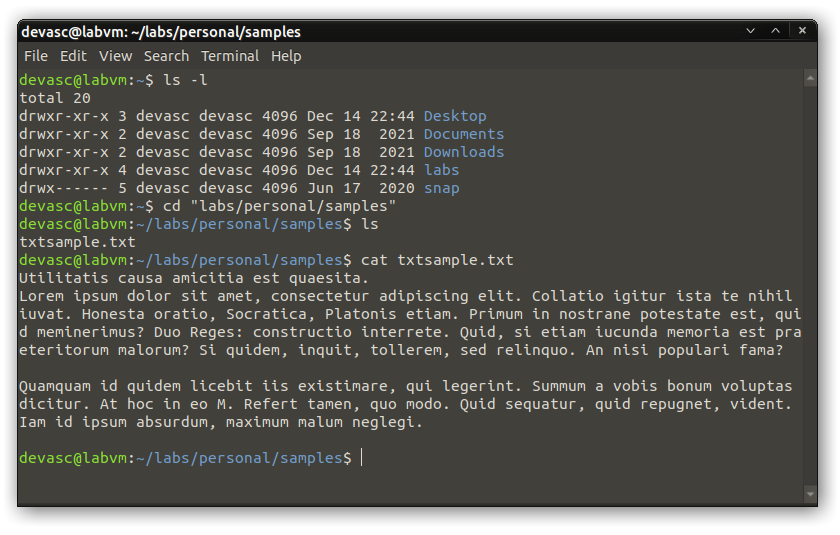
\includegraphics[height=4.7cm]{terminal-linux}
		\caption{Antarmuka perangkat lunak berbasis \cli.}
		\label{fig:commandline-cli}
	\end{subfigure}
	\hfill
    \begin{subfigure}[b]{0.5\linewidth}
		\centering
		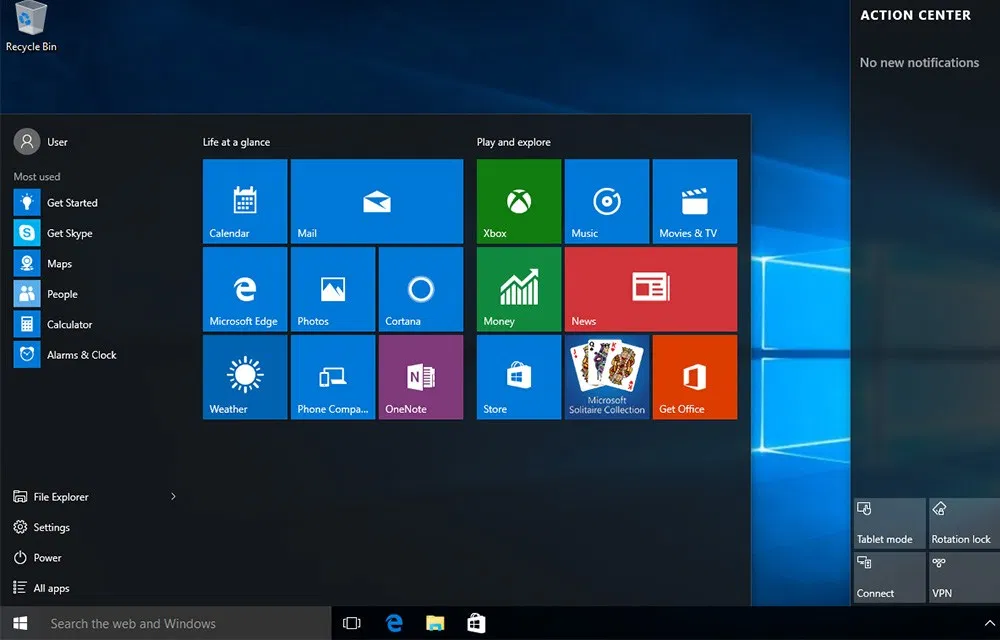
\includegraphics[height=4.33333cm]{gui}
		\caption{Antarmuka perangkat lunak berbasis \gui.}
		\label{fig:commandline-gui}
	\end{subfigure}
    \caption[Dua jenis tampilan perangkat lunak]{Contoh dua jenis antarmuka (\textit{interface)} perangkat lunak.}
	\label{fig:commandline-interfacetypes}
\end{figure}

Selain dari tampilannya sendiri, ada beberapa perbedaan utama lain antara perangkat-perangkat lunak berbasis \cli dengan perangkat lunak berbasis \gui. Adapun perbedaan-perbedaan utama dari kedua jenis antarmuka ini adalah sebagai berikut.\cite{mueller:2007:windowscommandline}
\begin{itemize}
	\item Pengunaan sumber daya sistem untuk menjalankan perangkat lunak berbasis \cli lebih rendah dibandingkan dengan perangkat lunak berbasis \gui.
	\item Bagi pengguna pemula (atau pengguna awam pada umumnya), perangkat lunak berbasis \cli akan lebih sulit digunakan karena tidak adanya bantuan apapun dalam bentuk visual, sehingga satu-satunya cara untuk tahu bagaimana cara menggunakan fitur-fiturnya adalah melalui dokumentasi perangkat lunak yang ada. Karena alasan yang sama pula, perangkat lunak berbasis \cli lebih sulit untuk dibiasakan penggunaannya.
	\item Automasi perintah yang bersifat berulang-ulang jauh lebih mudah dilakukan pada perangkat lunak berbasis \cli. Hal ini dikarenakan perangkat lunak berbasis \cli tidak hanya lebih mudah untuk dibuat \textit{script}-nya, tetapi juga lebih efisien untuk digunakan ketika ada banyak sekali perintah yang harus dilakukan pada suatu saat tertentu.
\end{itemize}

\subsection{\textit{Command Line} di Linux}
\label{sec:commandline-linux}

Linux merupakan sebuah sistem operasi yang sangat modular, jadi ada banyak sekali \textit{shell} yang dapat dijalankan dan digunakan di dalamnya. Walaupun begitu, ada satu \textit{shell} yang selalu datang ter-\textit{install} di dalam semua sistem operasi Linux, yaitu \textit{``bash''} (GNU \textit{\textbf{B}ourne \textbf{A}gain \textbf{Sh}ell}).\cite{matthew:2007:beginninglinuxprogramming}

\subsubsection{Tampilan}
\label{sec:commandline-linux-appearance}

Ketika terminal di Linux dijalankan, akan keluar kotak dialog, beserta sebuah baris. Baris ini biasanya berisi sebuah teks dengan format sebagai berikut.

\begin{verbatim}
        <nama pengguna>@<nama perangkat>:<direktori yang sedang diproses>$
\end{verbatim}

Tanda dolar di ujung baris ini menandakan bahwa baris tersebut merupakan baris \textit{shell prompt}, yang merupakan waktu di mana terminal sudah siap menerima masukan dari pengguna untuk diproses. Perlu diingat bahwa di posisi tanda dolar ini, terkadang justru terdapat tanda pagar (\#). Tanda pagar di akhir baris \textit{shell prompt} menandakan bahwa terminal tersebut dijalankan dengan tingkat akses \textit{superuser}, yang berarti bahwa entah pengguna masuk ke sistem sebagai user \textit{root}, atau terminal memiliki izin tingkat \textit{superuser/administrator}.\cite{shottsjr:2019:linuxcommandline}

\begin{figure}[ht]
    \begin{subfigure}[b]{0.475\linewidth}
		\centering
		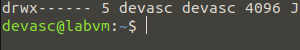
\includegraphics[width=\linewidth]{linux-shellprompt-normal}
		\caption{\textit{Shell prompt} terminal dengan tingkat izin \mbox{normal}.}
		\label{fig:shellprompt-linux-normal}
	\end{subfigure}
	\hfill
    \begin{subfigure}[b]{0.475\linewidth}
		\centering
		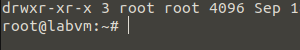
\includegraphics[width=\linewidth]{linux-shellprompt-superuser}
		\caption{\textit{Shell prompt} terminal dengan tingkat izin \textit{\mbox{superuser}}.}
		\label{fig:shellprompt-linux-superuser}
	\end{subfigure}
    \caption{Baris \textit{shell prompt} terminal di sistem operasi Linux.}
	\label{fig:commandline-shellprompt-linux}
\end{figure}

\subsubsection{Navigasi \cite{shottsjr:2019:linuxcommandline}}
\label{sec:commandline-linux-nav}

Sama seperti di Windows, Linux menyimpan file-filenya di sebuah struktur direktori yang bersifat hierarkial. Hal ini berarti bahwa file-file tersebut disimpan dalam direktori-direktori (atau \textit{folder-folder}) yang tersusun seperti sebuah pohon. dalam arti bahwa satu \textit{folder} bisa jadi berada di dalam satu \textit{folder} lain, atau berisi beberapa \textit{folder} lainnya.

Untuk navigasi, terminal Linux memiliki beberapa perintah utama. Adapun perintah-perintah tersebut adalah sebagai berikut.

\begin{itemize}
	\item \verb|pwd|\\
	\verb|pwd| merupakan singkatan dari \textit{print working directory}, yang berarti bahwa perintah ini akan mengeluarkan \textit{working directory}, atau direktori tempat terminal sekarang sedang bekerja/berjalan, sebagai keluaran dari perintah tersebut. Ketika pengguna pertama kali menjalankan terminal, \textit{working directory}-nya selalu merupakan direktori \textit{home} dari perangkat.
	\item \verb|ls|\\
	\verb|ls| digunakan untuk menghasilkan keluaran berupa isi dari folder yang dispesifikasi. Biasanya digunakan ketika pengguna sudah memasuki folder yang diinginkan, walaupun dengan perintah ini, pengguna bisa saja mengintip isi dari folder manapun di direktori manapun, dengan mengikutkan direktori yang diinginkan sebagai parameter dari perintah tersebut. Adapun Isi dari folder yang diikutkan sebagai parameter tidak hanya berupa folder lain, tetapi juga seluruh file-file yang ada, walaupun untuk file-file yang disembunyikan (nama file diawali dengan tanda titik), perlu ditambahkan opsi \verb|-a| agar file-file tersebut muncul pula dalam keluarannya.
	\item \verb|cd|\\
	\verb|cd| adalah perintah yang berfungsi untuk mengganti \textit{working directory} dari terminal. Untuk melakukan hal tersebut, perintah yang perlu dimasukkan adalah sebagai berikut:
	
	\begin{verbatim}
	                     cd <direktori yang diinginkan>
	\end{verbatim}
	
	Direktori yang diinginkan dapat berupa direktori absolut, atau direktori relatif. Perbedaannya adalah direktori absolut selalu dimulai dari folder \textit{root}, mengikuti folder-folder apapun yang ada di antara \textit{root} sampai ke folder yang diinginkan.
	
	Sedangkan, direktori relatif selalu dimulai dari \textit{working directory}. Untuk penggunaan direktori relatif, diperlukan dua buah notasi spesial, yaitu titik (\verb|.|), yang merepresentasikan \textit{working directory} sekarang itu sendiri, dan dua titik (\verb|..|), yang merepresentasikan \textit{parent folder} dari \textit{working directory}.
\end{itemize}

\subsubsection{\texttt{man} \cite{shottsjr:2019:linuxcommandline}}
\label{sec:commandline-linux-manpage}

Untuk sistem-sistem operasi berbasis Linux, ada sebuah konvensi bahwa semua perangkat lunak \textit{executable} yang dimaksudkan untuk dijalankan melalui \cl perlu disertai dengan sebuah dokumentasi formal yang disebut \textit{manual} atau \textit{man page}. Di sistem-sistem operasi ini sudah ada perangkat lunak khusus, bernama ``\textit{man}'' yang fungsinya adalah untuk menampilkan dokumentasi-dokumentasi ini. Adapun \textit{man} digunakan dengan perintah berikut:

\begin{verbatim}
                           man <nama perangkat lunak>
\end{verbatim}
\noindent
\textit{Man page} tidak memiliki format umum, tapi pada umumnya memiliki bagian-bagian berikut:

\begin{itemize}
	\item judul\textemdash perangkat lunak mana yang sedang ditampilkan halaman \textit{man}-nya,
	\item perintah penggunaan perangkat lunak,
	\item deskripsi singkat dari fungsi perangkat lunak, serta
	\item daftar fitur-fitur perangkat lunak serta cara penggunaannya.
\end{itemize}
\noindent
Walaupun begitu, perlu diingat bahwa halaman \textit{man} umumnya tidak mengikutkan contoh penggunaan. Selain itu, perlu juga diingat bahwa halaman \textit{man} ini dibagi ke delapan bagian, di mana bagian-bagiannya dapat dilihat di tabel \ref{tab:commandline-linux-manpage-sections}.

\begin{table}[H]
    \centering
    \begin{tabular}{| c | c |}
    \hline
        \textbf{Bagian} & \textbf{Kategori \textit{manual}} \\
    \hline
    \hline
        1 & Perintah pengguna \\
    \hline
        2 & Panggilan langsung ke \textit{kernel} sistem \\
    \hline
        3 & Panggilan langsung ke \textit{library} C \\
    \hline
        4 & File-file spesial (contohnya \textit{driver}) \\
    \hline
        5 & Format file \\
    \hline
        6 & Permainan \\
    \hline
		7 & Lain-lain \\
	\hline
		8 & Perintah administrasi sistem \\
	\hline
	\end{tabular}
    \caption{Jumlah kategori dan tes yang dilakukan.}
    \label{tab:commandline-linux-manpage-sections}
\end{table}
\noindent
Adapun contoh penggunaan perintah \texttt{man} ini ada di gambar <REF!>.

\subsection{\textit{Command Line} di Windows}
\label{sec:commandline-windows}

Cara kerja \cl di Windows serupa dengan cara kerja \cl di Linux, dalam arti bahwa untuk bekerja dengan \cl di Windows, penggunanya juga akan langsung berinteraksi dengan utilitas yang disediakan oleh sistem operasi. \textit{Command line} di Windows juga dapat digunakan untuk hal-hal yang serupa dengan \cl di Linux, seperti menulis (dan menjalankan) \textit{script}, menjalankan perintah yang diinginkan pengguna secara otomatis, atau melihat status dari sistem operasi.\cite{mueller:2007:windowscommandline}

Masih sama dengan Linux, ada banyak sekali command yang bisa digunakan, sehingga susah untuk menghafal seluruh command-command yang ada\textemdash termasuk masukan, parameter-parameter yang dibutuhkan, serta keluarannya. Untuk melihat dokumentasi, atau penjelasan detail untuk masukan, keluaran, parameter, serta opsi-opsi dari perintah tertentu, pengguna dapat memasukkan perintah tersebut, diikuti dengan \verb|/?|.\cite{mueller:2007:windowscommandline}

\subsubsection{Tampilan}
\label{sec:commandline-windows-appearance}

Di sistem operasi Windows, ada dua jenis antarmuka \cl, yaitu cmd (\textit{Command Prompt}) dan \textit{PowerShell}. Keduanya memiliki tampilan yang kurang lebih sama\textemdash hanya saja awalnya cmd memiliki latar belakang hitam, sedangkan \textit{PowerShell} memiliki latar belakang biru tua, seperti terlihat di gambar \ref{fig:commandline-windows-programs}.

\begin{figure}[ht]
    \begin{subfigure}[b]{0.49\linewidth}
		\centering
		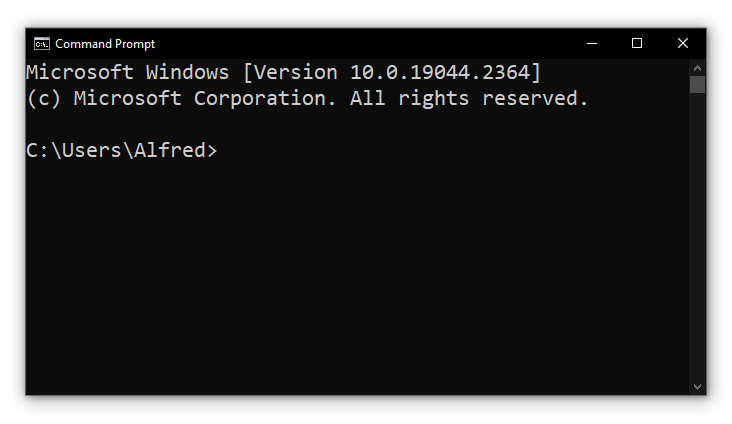
\includegraphics[width=\linewidth]{windows-cmd}
		\caption{Antarmuka Windows \textit{Command Prompt} (\textit{cmd})}
		\label{fig:commandline-windows-cmd}
	\end{subfigure}
	\hfill
    \begin{subfigure}[b]{0.49\linewidth}
		\centering
		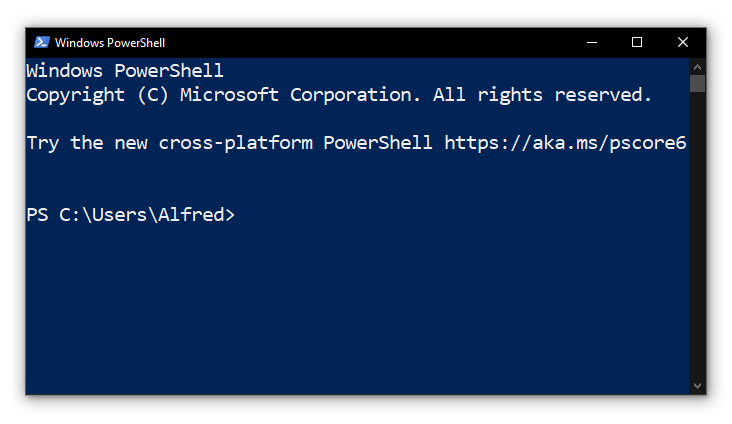
\includegraphics[width=\linewidth]{windows-powershell}
		\caption{Antarmuka Winodws \textit{PowerShell}}
		\label{fig:commandline-windows-powershell}
	\end{subfigure}
    \caption{Tampang kedua antarmuka \cl bawaan di sistem operasi Windows.}
	\label{fig:commandline-windows-programs}
\end{figure}

\subsubsection{Navigasi}
\label{sec:commandline-windows-nav}

Untuk navigasi di antarmuka \cl Windows, ada dua perintah penting yang dipakai ketika pengguna sedang berurusan dengan file-file dan navigasi dalam direktori sistem. Kedua perintah tersebut adalah \verb|cd| dan \verb|dir|.

\begin{itemize}
	\item \verb|cd| (\verb|chdir|) \cite{microsoftdocs:2021:windowscommands}\\
	\verb|cd| merupakan sebuah perintah yang memiliki tiga fungsi utama, yaitu menampilkan \textit{drive} tempat sedang \cl berada (jika pengguna hanya memasukkan \verb|cd| tanpa parameter apapun), menampilkan direktori tempat \cl sedang berada (jika pengguna hanya memasukkan \textit{drive} sebagai parameter, atau fungsi yang paling umumnya, untuk mengganti \textit{working directory} dari \cl.
	\newline\newline
	Adapun format dari perintah \verb|dir| adalah sebagai berikut.
	
	\begin{verbatim}
                        cd [/d] [<drive>:][<path>]
	\end{verbatim}
	
	Dengan fungsi dari semua opsi dan parameter yang ada sebagai berikut.
	
	\begin{itemize}
		\item \verb|/d|\\
		Opsi yang menandakan bahwa pengguna ingin mengganti \textit{drive} (partisi) dan juga \textit{working directory} dari \cl.
		\item \verb|<drive>:|\\
		Kode huruf dari partisi yang akan diproses.
		\item \verb|<path>|\\
		Direktori yang akan diproses. Parameter ini harus diikutkan beserta kode huruf partisi (tidak dapat berdiri sendiri.)
	\end{itemize}
	
	\item \verb|dir|\\
	\verb|dir| merupakan sebuah perintah yang mengeluarkan/menampilkan sebuah daftar berisi file-file yang ada di suatu direktori, termasuk subdirektori. Jika tidak disertai parameter apapun, perintah ini akan menampilkan label volume dan nomor serial \textit{disk}, dilanjutkan dengan daftar direktori dan file di dalamnya. Untuk file, akan ditampilkan nama beserta ukurannya. Perintah ini juga akan menampilkan jumlah direktori dan file yang didaftarkan, ukuran kumulatifnya, dan sisa dari \textit{disk} yang tidak terpakai (dalam \textit{bytes}).\cite{microsoftdocs:2021:windowscommands}
	\newline\newline
	Adapun format dari perintah \verb|dir| adalah sebagai berikut.\cite{mueller:2007:windowscommandline}
	
	\begin{verbatim}
         dir [<drive:>][<path>][<filename>] [/A[[:]<attributes>]] [/B] 
         [/C] [/D] [/L] [/N] [/O[[:]<sortorder>]] [/P] [/Q] [/R] [/S] 
                    [/T[[:]<timefield>]] [/W] [/X] [/4]
	\end{verbatim}
	
	Untuk perintah ini, seperti terlihat di atas, memiliki banyak sekali opsi dan parameter. Tiap-tiap dari parameter tersebut memiliki fungsi tersendiri, yaitu:
	\begin{itemize}
		\item \verb|/A[[:]<attributes>]|\\
		Menampilkan file-file dengan atribut tertentu, seperti file yang disembunyikan, file sistem, file \textit{read-only}, dan sebagainya.
		\item \verb|/B|\\
		Menghilangkan \textit{heading} dan ringkasan informasi dari keluaran, atau dengan kata lain, hanya menampilkan file-file dan direktori, tanpa informasi tambahan apapun.
		\item \verb|/C|\\
		Menggunakan separator koma untuk tiap angka ribuan di ukuran file. Jika opsi yang dimasukkan adalah \verb|/-C|, separator koma justru akan dihilangkan.
		\item \verb|/D|\\
		Menampilkan keluaran dengan format yang lebih lebar. Jika opsi ini diikutkan, keluaran akan ditampilkan dengan urutan berdasarkan kolom.
		\item \verb|/L|\\
		Seluruh teks dalam keluaran akan menggunakan huruf kecil. Jika opsi ini tidak digunakan, keluaran akan mengandung huruf besar dan huruf kecil \textit{mixed case}.
		\item \verb|/N|\\
		Menampilkan daftar dengan format panjang, dengan nama file berada di ujung paling kanan.
		%\newpage \enlargethispage{1.5\baselineskip} % Prevent widow
		\item \verb|/O[[:]<sortorder>]|\\
		Menampilkan daftar direktori yang terurut berdasarkan urutan tertentu, seperti berdasarkan ekstensi file, berdasarkan tanggal dibuat, berdasarkan nama, dan sebagainya. Jika tidak diikutkan tanda minus (\verb|-|) sebelum huruf \verb|O| pada perintah, daftar yang muncul akan terurut secara menaik.
		\item \verb|/P|\\
		Memberhentikan keluaran selama beberapa waktu singkat (memberi jeda kecil) setelah setiap halaman informasi.
		\item \verb|/Q|\\
		Menambahkan informasi mengenai pemilik file dalam keluaran.
		\item \verb|/R|\\
		Menampilkan \textit{data stream} alternatif, jika ada.
		\item \verb|/S|\\
		Mendaftarkan seluruh file di direktori dan subdirektori yang diproses. Tiap-tiap direktori akan memiliki \textit{header} tersendiri dalam keluarannya.
		\item \verb|/T[[:]<timefield>]|\\
		Menspesifikasi \textit{time field} mana yang akan tampil dan digunakan sebagai urutan, jika aturan pengurutan lain tidak ditentukan. \textit{Time field} yang dapat digunakan adalah waktu pembuatan file, kapan terakhir file diakses, dan kapan file terakhir dimodifikasi. Jika parameter ini tidak dispesifikasi, \textit{time field} yang digunakan adalah kapan file terakhir dimodifikasi.
		\item \verb|/W|\\
		Menampilkan keluaran dengan format yang lebih lebar. Opsi ini hampir sama dengan \verb|/D|, hanya saja untuk \verb|/W|, jika opsi ini diikutkan, keluaran akan ditampilkan dengan urutan berdasarkan baris, dan bukan kolom.
		\item \verb|/X|\\
		Menampilkan nama pendek yang dibuat untuk nama-nama file non-8.3. Opsi ini memiliki format taampilan yang sama seperti opsi \verb|/N|, hanya saja nama pendeknya ditampilkan di keluaran sebelum nama panjangnya.
		\item \verb|4|\\
		Menampilkan angka tahun dengan format angka empat digit.
	\end{itemize}
\end{itemize}

\section{KIRI}
\label{sec:kiri}

KIRI merupakan sebuah perangkat lunak berbasis web yang berfungsi untuk menyelesaikan (atau setidaknya mengurangi) dampak dari masalah-masalah yang dapat diselesaikan oleh transportasi umum/publik di Indonesia, seperti pemanasan global, kemacetan, atau peningkatan harga bensin. Selain itu, turis mancanegara juga memilih untuk menaiki transportasi umum, karena jenis sarana transportasi tersebut tidak hanya jauh lebih murah, tetapi juga memberikan kesempatan yang mudah kepada mereka untuk melihat seluk-beluk dari kota-kota yang mereka kunjungi. Walaupun begitu, banyak masyarakat lokal sendiri yang seringkali masih segan untuk menaiki transportasi publik, umumnya karena transportasi publik dianggap lebih rumit persiapannya dibandingkan dengan metode-metode transportasi privat, seperti menaiki kendaraan pribadi.\footnote{\href{https://projectkiri.github.io/\#about-kiri}{https://projectkiri.github.io/\#about-kiri}}

Di halaman web KIRI, pengguna dapat memasukkan input berupa lokasi awal dan lokasi tujuan dan KIRI akan menghasilkan seluruh langkah yang harus ditempuh oleh pengguna untuk sampai ke lokasi tujuan, dengan menggunakan angkot. Keluaran ini sudah meliputi kode angkot mana saja yang harus dinaiki, dan juga seberapa jauh pengguna harus berjalan kaki untuk sampai ke lokasi rute angkot berikutnya.

\subsection{Tampilan}
\label{sec:kiri-appearance}

Pada saat pertama kali dibuka, hal pertama yang paling mencolok di halaman awal web KIRI adalah sebuah peta besar di sebelah kiri yang dapat diperbesar ataupun diperkecil. Sedangkan, bagian kanan dari halamannya terdiri atas beberapa bagian. Di bagian paling atas terdapat logo KIRI, beserta sepasang menu \textit{dropdown}\textemdash yang pertama merupakan pilihan kota tempat pengguna berada (untuk sekarang hanya tersedia pilihan kota Jakarta dan Bandung), dan yang kedua merupakan pilihan bahasa, entah bahasa Indonesia atau Inggris. Di bawahnya merupakan sepasang menu \textit{dropdown} yang merupakan tempat di mana pengguna memasukkan lokasi awal dan tujuan yang akan diproses oleh KIRI. Terakhir, di bawahnya ada sebuah bagian kosong, yang nantinya akan menjadi tempat di mana KIRI akan meletakkan keluaran dari prosesnya. Adapun tampilan awal dari halaman web ini dapat dilihat di gambar \ref{fig:kiri-base}.

\begin{figure}[ht]
    \centering
    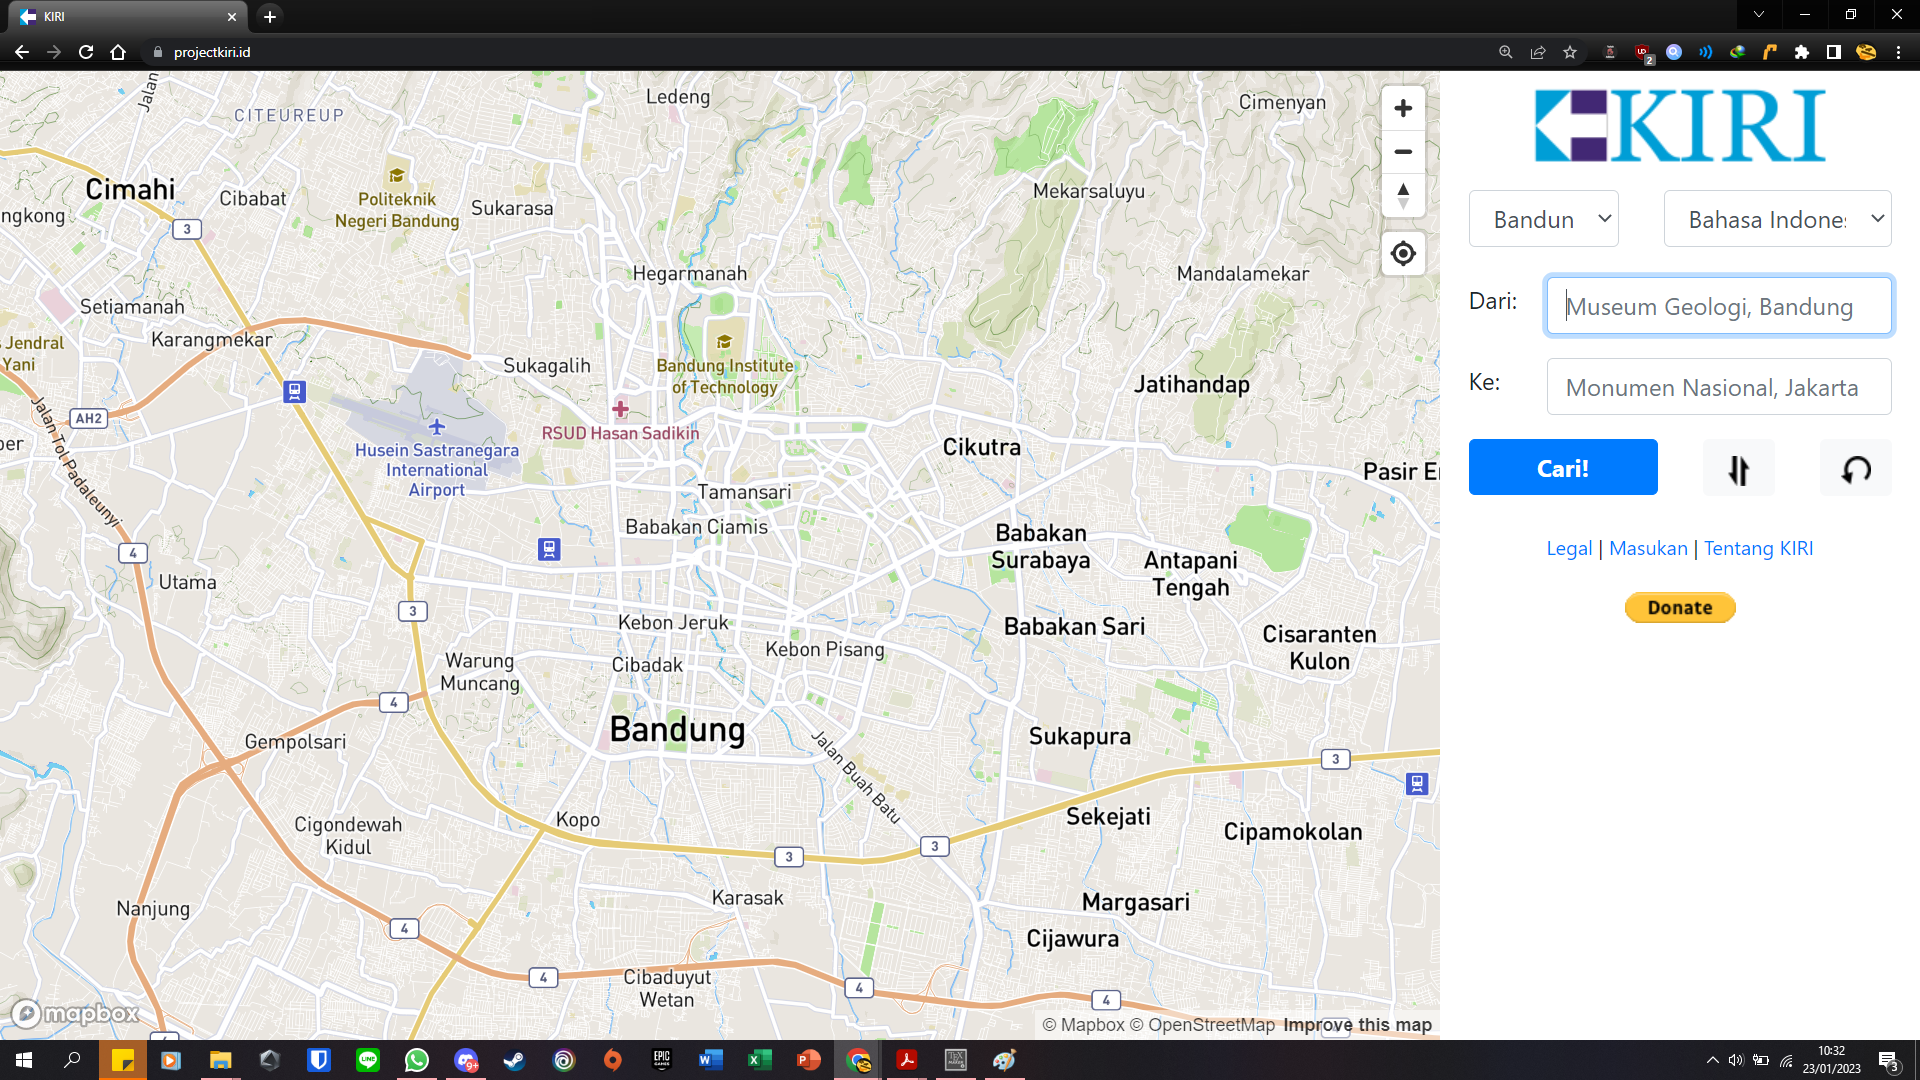
\includegraphics[width=0.74\linewidth]{projectkiri-base}
    \caption[Tampilan awal halaman web KIRI]{Tampilan awal halaman web KIRI.}
    \label{fig:kiri-base}
\end{figure}

Ada dua area yang memiliki perbedaan yang signifikan ketika pengguna sudah memasukkan masukan dan menyuruh KIRI untuk memprosesnya. Bagian yang pertama adalah bagian peta, yang setelah pemrosesan masukan, akan memiliki garis-garis berwarna yang menandakan rute angkot maupun tujuan perjalanan kaki yang harus ditempuh oleh pengguna. Bagian kedua adalah bagian keluaran, yang tadinya kosong, sekarang akan berisi langkah-langkah yang harus ditempuh oleh penggunanya untuk pergi dari lokasi awal ke lokasi tujuan. Spesifiknya, perbedaan-perbedaan ini dapat dilihat di gambar \ref{fig:kiri-example}.

\begin{figure}[ht]
    \centering
    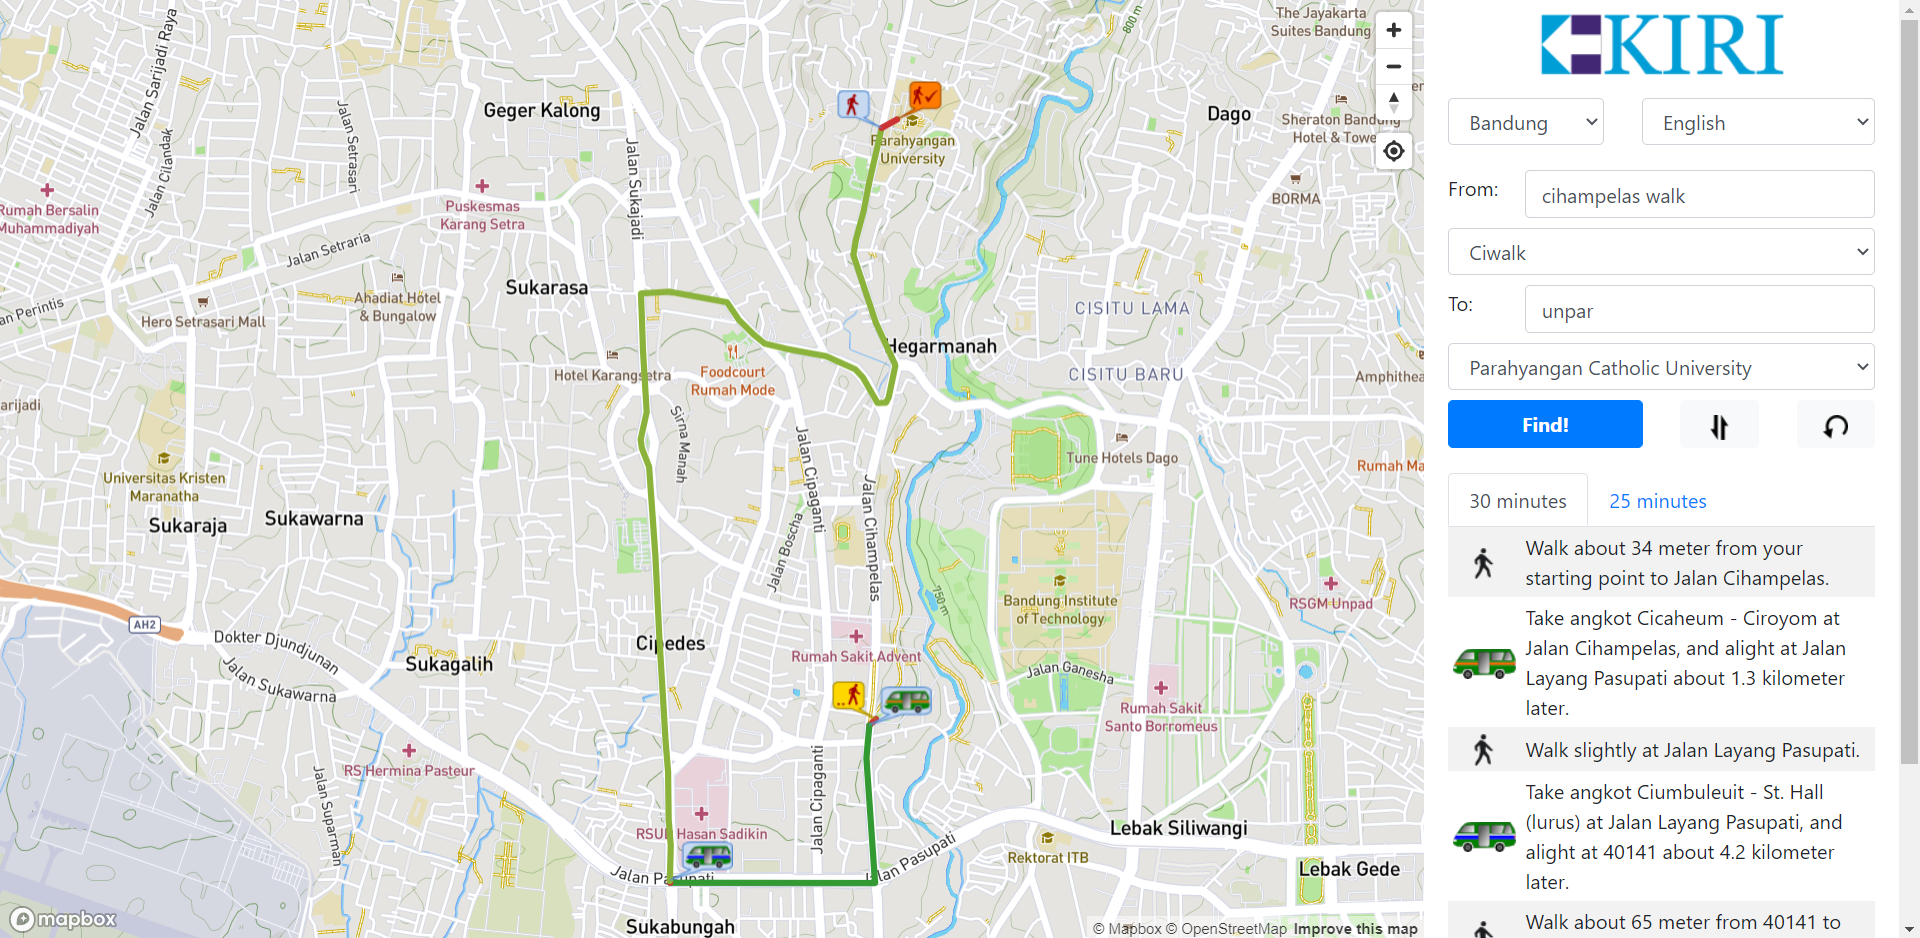
\includegraphics[width=0.74\linewidth]{projectkiri-example}
    \caption[Tampilan akhir halaman web KIRI]{Tampilan halaman web KIRI setelah pemrosesan masukan dari pengguna selesai.}
    \label{fig:kiri-example}
\end{figure}

%\newpage
\subsection{API\protect\footnotemark}
\label{sec:kiri-api}
\footnotetext{\href{https://github.com/projectkiri/Tirtayasa/wiki/KIRI-API-v2}{https://github.com/projectkiri/Tirtayasa/wiki/KIRI-API-v2}}

KIRI juga memiliki sebuah API yang dapat digunakan untuk keperluan pengembangan perangkat lunak. API ini menyediakan tiga buah jenis layanan web (\textit{webservice}), yang ketiganya dapat dilakukan dengan mengirim pemintaan (\textit{request}) tipe GET melalui API tersebut. Isi dari permintaan yang perlu dikirimkan serta respon dari API yang akan dikembalikan berbeda tergantung dari jenis layanan yang digunakan. Adapun ketiga jenis layanan tersebut adalah pencarian tempat (\textit{search place}), pencarian rute (\textit{routing}), dan \textit{smart direction}.
 
\subsubsection{\textit{Search Place}}
\label{sec:kiri-api-searchplace}

Layanan pencarian lokasi (\textit{search place}) adalah layanan web pada API KIRI yang berfungsi untuk mencari suatu lokasi berdasarkan kata kunci yang diberikan oleh pengguna. Untuk menggunakan layanan ini, pengguna harus mengirim permintaan GET ke alamat \href{https://projectkiri.id/api}{https://projectkiri.id/api}. Adapun permintaan tersebut harus memiliki parameter-parameter seperti terlihat di bawah ini.

\begin{itemize}
	\item \verb|version|\\
	\textbf{Kemungkinan nilai:} \verb|2|\\
	Parameter ini merupakan tanda bagi API untuk menggunakan protokol versi 2.
	\item \verb|mode|\\
	\textbf{Kemungkinan nilai:} \verb|searchplace|\\
	Parameter ini merupakan mode dari servis/jasa API yang akan digunakan oleh pengguna. Untuk pengunaan layanan pencarian lokasi, variabel ini harus diisi dengan \verb|searchplace|.
	\item \verb|region|\\
	\textbf{Kemungkinan nilai:} \verb|cgk|, \verb|bdo|, \verb|mlg|, atau \verb|sub|\\
	Parameter ini merupakan kode bandara IATA tiga huruf yang merepresentasikan daerah mana tempat lokasi yang ingin dicari berada. Kode yang dapat diproses oleh API ini meliputi \verb|cgk| (Cengkareng/Jakarta), \verb|bdo| (Bandung), \verb|mlg| (Malang), dan \verb|sub| (Surabaya).
%	\newpage % Prevent widow
	\item \verb|querystring|\\
	\textbf{Kemungkinan nilai:} \textit{string} berisi teks apapun dengan panjang minimal satu karakter\\
	Parameter ini berisi kata kunci yang akan digunakan untuk menentukan lokasi yang ingin dicari pengguna.
	\item \verb|apikey|\\
	\textbf{Kemungkinan nilai:} angka heksadesimal 16-digit\\
	Parameter ini berisi kunci API pribadi yang harus digenerasi terlebih dahulu sebelum API dapat digunakan.
\end{itemize}
\vspace{\baselineskip}
Perlu diperhatikan bahwa salah satu dari parameter yang harus diikutkan dalam pesan tersebut merupakan parameter yang meminta kunci API. Kunci tersebut harus digenerasikan terlebih dahulu sebelum API KIRI dapat digunakan, melalui halaman \textit{API Keys} KIRI,\footnote{\href{https://projectkiri.id/dev/apikeys}{https://projectkiri.id/dev/apikeys}} yang dapat dilihat di gambar \ref{fig:kiri-apikeypage}.

\begin{figure}[t]
    \centering
    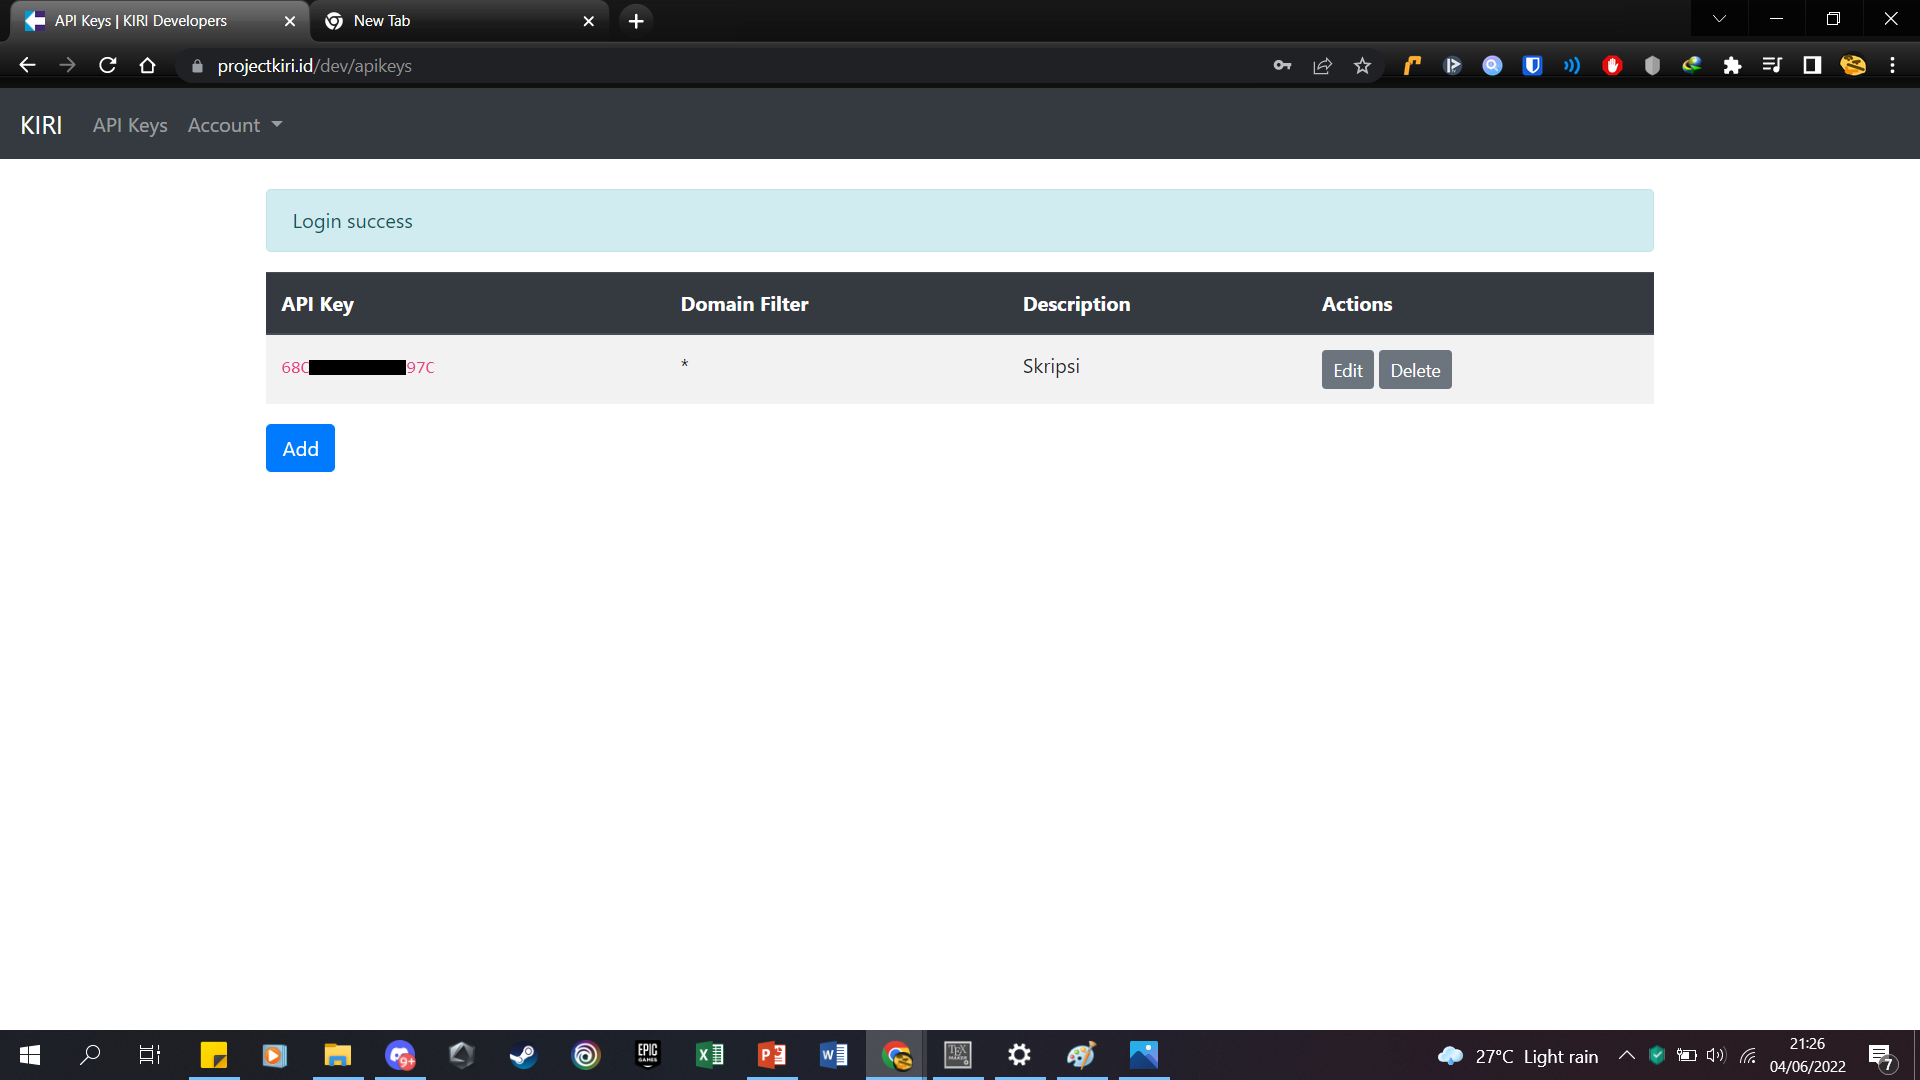
\includegraphics[width=0.75\linewidth]{projectkiri-apikey}
    \caption[Halaman web \textit{API Keys} KIRI.]{Halaman web \textit{API Keys} KIRI.}
    \label{fig:kiri-apikeypage}
\end{figure}

Untuk mengakses halaman tersebut, pengguna harus membuat sebuah akun terlebih dahulu. Ketika akun sudah dibuat, maka pengguna baru akan dapat membuat kunci API yang dibutuhkan, sekaligus membuat filter \textit{domain}, yang membatasi di \textit{domain} mana saja kunci tersebut dapat digunakan, serta memberikan deskripsi untuk kunci API tersebut. Kunci ini kemudian dapat digunakan sebagai nilai dari parameter \verb|apikey| yang diperlukan dalam permintaan tadi.

Sebelum membahas keluaran dari layanan API ini, perlu ditegaskan dulu apa definisi dari nilai \latlon suatu lokasi. \textit{Latitude} merupakan berapa derajat sebuah tempat berada dari garis ekuator, dengan lokasi-lokasi yang berada maksimum 90 derajat di atas ekuator memiliki nilai \textit{latitude} positif, sedangkan lokasi-lokasi yang berada maksimum 90 derajat di bawah ekuator memiliki nilai \textit{latitude} negatif. Sedangkan, \textit{longitude} merupakan berapa derajat lokasi sebuah tempat berada dari garis meridian (bujur) utama Bumi, dengan rentang nilai dari -180 derajat di sisi kiri (barat) meridian utama, hingga 180 derajat di kanan (timur) bujur tersebut.\footnote{\href{https://gsp.humboldt.edu/olm/Lessons/GIS/01\%20SphericalCoordinates/Latitude\_and\_Longitude.html}{https://gsp.humboldt.edu/olm/Lessons/GIS/01\%20SphericalCoordinates/Latitude\_and\_Longitude.html}} Kedua nilai ini merupakan salah satu dari dua variabel yang dikembalikan dalam respon API untuk layanan ini, dengan variabel lainnya berupa nama dari lokasi yang ditemukan itu sendiri. Adapun respon yang diberikan oleh API akan berupa sebuah objek JSON yang selalu memiliki setidaknya dua variabel, yaitu:

\begin{itemize}
	\item \verb|status|\\
	\textbf{Kemungkinan nilai:} \verb|ok| atau \verb|error|\\
	Variabel ini manandakan apakah permintaan berhasil diproses atau tidak. Jika permintaan berhasil diproses, variabel ini akan bernilai \verb|ok|, dan jika tidak, variabel ini akan bernilai \verb|error|.
	\item \verb|message|\\
	Variabel ini bisa berisi dua macam objek. Jika permintaan dari user tidak berhasil diproses, atau dalam kata lain, terjadi sebuah \textit{error}, maka variabel ini akan berisi string yang merupakan pesan \textit{error} serta alasan spesifik mengapa \textit{error} tersebut terjadi. Di lain sisi, jika permintaan dari pengguna berhasil diproses, variabel ini akan mengalami dua perubahan utama. Pertama, nama variabel ini akan berubah menjadi \verb|searchresult|, dan kedua, isi dari variabel ini akan menjadi sebuah \textit{array} yang merupakan respon dari API KIRI berupa keluaran yang akan dilihat oleh pengguna. \textit{Array} ini sendiri akan memiliki variabel berikut.
	
	\begin{itemize}
		\item \verb|placename|\\
		Variabel ini berisi nama lokasi yang ditemukan berdasarkan kata kunci yang diberikan oleh pengguna.
		\item \verb|location|\\
		Variabel ini berisi nilai \latlon dari lokasi yang ditemukan dalam pencarian.
	\end{itemize}
	
\end{itemize}
\vspace{\baselineskip}\noindent
Contoh dari penggunaan API KIRI untuk layanan ini dapat dilihat di gambar \ref{fig:kiri-api-searchplace-usage}.

\begin{figure}[t]
    \centering
    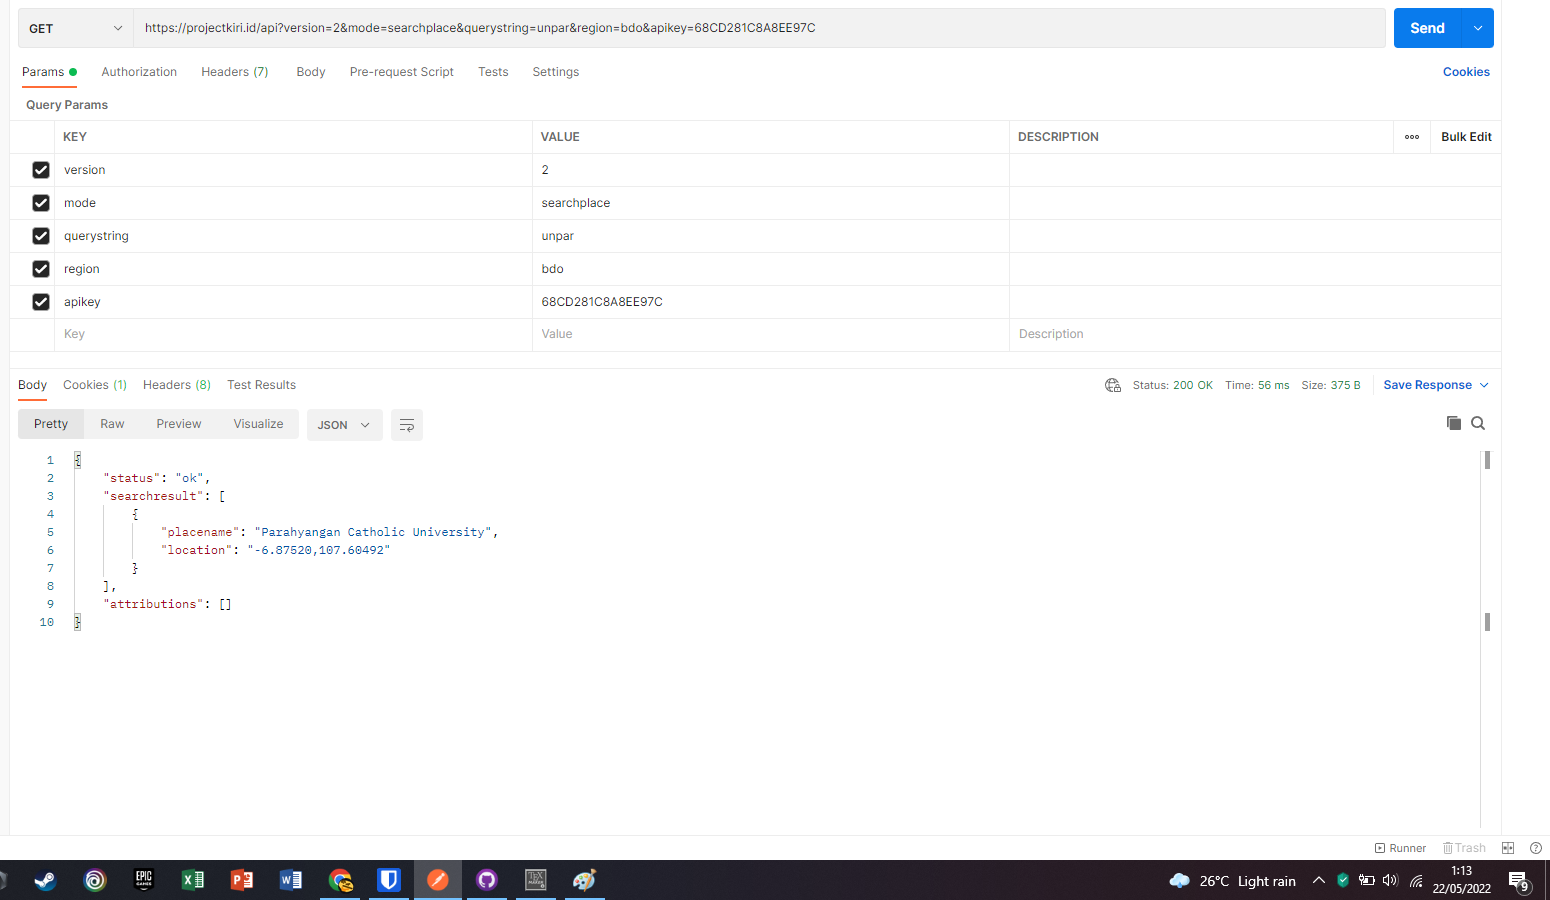
\includegraphics[width=0.74\linewidth]{apikiri-searchplace}
    \caption[Penggunaan API KIRI untuk layanan pencarian lokasi]{Penggunaan API KIRI untuk layanan pencarian lokasi menggunakan Postman. Gambar ini menunjukkan hasil pencarian lokasi ``unpar'' di daerah Bandung.}
    \label{fig:kiri-api-searchplace-usage}
\end{figure}

\subsubsection{\textit{Routing}}
\label{sec:kiri-api-routing}

Layanan pencarian rute (\textit{routing}) adalah layanan web pada API KIRI yang memiliki fungsi yang sama dengan fungsi utama dari perangkat lunak KIRI sendiri, yaitu menunjukkan rute serta langkah-langkah yang harus ditempuh untuk pergi dari satu lokasi ke lokasi lainnya, dengan menggunakan angkot yang tersedia. Untuk menggunakan layanan ini, pengguna harus mengirim permintaan GET ke alamat \href{https://projectkiri.id/api}{https://projectkiri.id/api}. Adapun permintaan tersebut harus memiliki parameter-parameter seperti terlihat di bawah ini.
%\newpage % Prevent widow
\begin{itemize}
	\item \verb|version|\\
	\textbf{Kemungkinan nilai:} \verb|2|\\
	Parameter ini merupakan tanda bagi API untuk menggunakan protokol versi 2.
	\item \verb|mode|\\
	\textbf{Kemungkinan nilai:} \verb|findroute|\\
	Parameter ini merupakan mode dari servis/jasa API yang akan digunakan oleh pengguna. Untuk pengunaan layanan pencarian rute dengan angkot, variabel ini diisi dengan \verb|findroute|.
	\item \verb|locale|\\
	\textbf{Kemungkinan nilai:} \verb|en| atau \verb|id|\\
	Parameter ini mengatur bahasa apa yang akan digunakan dalam keluaran API nantinya\textemdash\verb|en| berarti keluaran akan menggunakan bahasa Inggris, dan \verb|id| berarti keluaran akan menggunakan bahasa Indonesia.
	\item \verb|start|\\
	\textbf{Kemungkinan nilai:} \verb|lat|, \verb|lng|; dalam bentuk desimal 10-digit\\
	Parameter ini merupakan nilai \latlon dari titik awal perjalanan pengguna.
	\item \verb|finish|\\
	\textbf{Kemungkinan nilai:} \verb|lat|, \verb|lng|; dalam bentuk desimal 10-digit\\
	Parameter ini berisi nilai \latlon dari titik akhir/tujuan perjalanan pengguna.
	\item \verb|presentation| (opsional)\\
	\textbf{Kemungkinan nilai:} \verb|desktop|\\
	Parameter ini hanya digunakan untuk fitur \textit{backwards compatibility}.
	\item \verb|apikey|\\
	\textbf{Kemungkinan nilai:} angka heksadesimal 16-digit\\
	Parameter ini berisi kunci API pribadi yang harus digenerasi terlebih dahulu sebelum API dapat digunakan.
\end{itemize}
\vspace{\baselineskip}
Sedangkan, respon yang diberikan oleh API akan berupa sebuah objek JSON yang selalu memiliki setidaknya dua variabel, yaitu:

\begin{itemize}
	\item \verb|status|\\
	\textbf{Kemungkinan nilai:} \verb|ok| atau \verb|error|\\
	Variabel ini manandakan apakah permintaan berhasil diproses atau tidak. Jika permintaan berhasil diproses, variabel ini akan bernilai \verb|ok|, dan jika tidak, variabel ini akan bernilai \verb|error|.
	\item \verb|message|\\
	Mirip dengan fitur \verb|searchplace|, jika permintaan dari pengguna tidak berhasil diproses, variabel ini akan berupa \textit{string} yang berisi pesan error dari API. Jika permintaan dari pengguna berhasil diproses, nama variabel ini akan berubah menjadi \verb|routingresults|, dan isi dari variabel ini akan menjadi sebuah \textit{array} JSON yang berisi variabel-variabel sebagai berikut:
	\begin{itemize}
		\item \verb|steps|\\
		\textbf{Tipe:} \textit{array}\\
		Variabel ini merepresentasikan satu buah langkah yang harus ditempuh oleh pengguna. Adapun \textit{array} ini sendiri berisi variabel-variabel berikut:
		
		\begin{itemize}
			\item Tipe transportasi\\
			Tipe sarana transportasi yang harus dipakai oleh pengguna. Jika pengguna harus berjalan kaki, variabel ini akan berisi \verb|walk|. Jika pengguna harus menaiki angkot, variabel ini akan berisi \verb|angkot|.
			\item Kode angkot\\
			Variabel ini menunjukkan angkot mana yang harus dinaiki oleh pengguna di langkah tersebut. Jika penggunaan angkot tidak dimungkinkan pada langkah ini (pengguna harus berjalan kaki), variabel ini akan berisi \verb|walk|.
			\item \textit{Array} \latlon lokasi\\
			\textit{Array} nilai-nilai desimal \latlon dari berbagai titik lokasi yang terdapat dalam rute.
			\item Deskripsi langkah\\
			Deskripsi langkah yang harus ditempuh, dalam bahasa natural. Bahasa yang digunakan tergantung parameter \verb|locale| yang diatur dalam masukan.
			\item URL untuk mendapatkan tiket kendaraan\\
			Tautan untuk mendapatkan tiket angkutan umum, jika diperlukan. Jika transportasi pada langkah tersebut tidak memerlukan tiket, variabel ini akan berisi \verb|null|.
			\item URL editor rute\\
			Tautan untuk melakukan modifikasi rute, jika dimungkinkan. Jika rute tidak bisa dimodifikasi, variabel ini akan berisi \verb|null|.
		\end{itemize}
		
		\item \verb|traveltime|\\
		\textbf{Tipe:} string\\
		Variabel ini berisi estimasi jangka waktu yang diperlukan untuk menyelesaikan langkah tersebut.
	\end{itemize}
	
\end{itemize}
\vspace{\baselineskip}\noindent
Adapun gambar \ref{fig:kiri-api-routing-usage} menunjukkan penggunaan API KIRI untuk layanan pencarian rute dari Cihampelas Walk ke Universitas Katolik Parahyangan.

\begin{figure}[t]
    \centering
    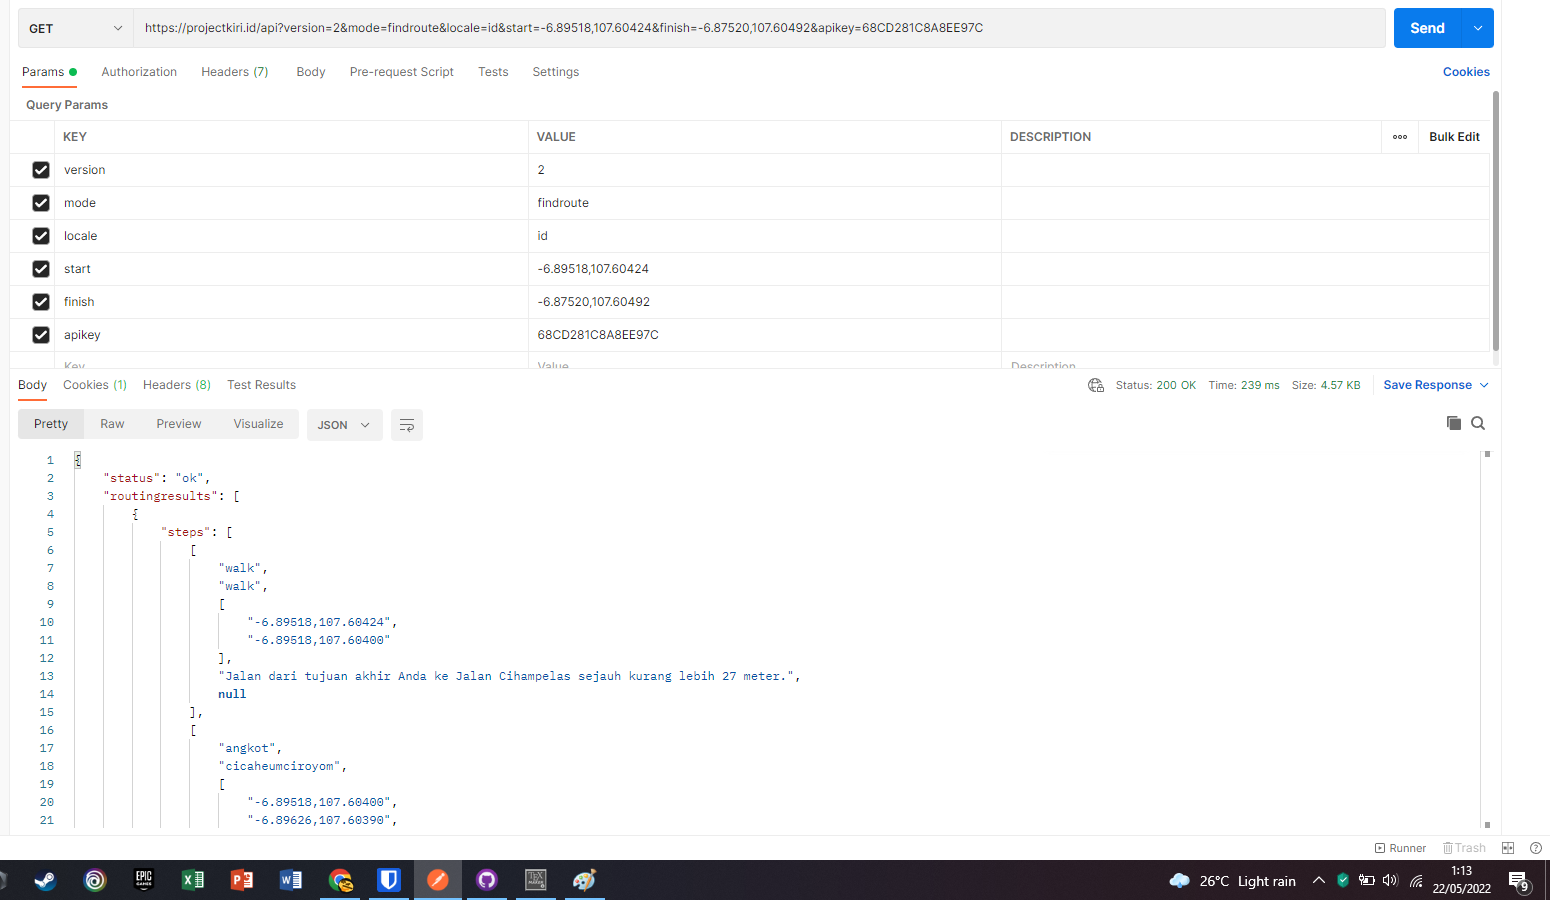
\includegraphics[width=0.74\linewidth]{apikiri-routing}
    \caption[Penggunaan API KIRI untuk layanan pencarian rute]{Penggunaan API KIRI untuk layanan pencarian rute menggunakan Postman. Gambar ini menunjukkan hasil pencarian rute dari Cihampelas Walk ke UNPAR.}
    \label{fig:kiri-api-routing-usage}
\end{figure}

\subsubsection{\textit{Smart Direction}}
\label{sec:kiri-api-smartdir}

Layanan terakhir dari API ini adalah layanan \textit{smart direction}, yang merupakan gabungan dari kedua layanan sebelumnya. Berbeda dengan kedua layanan tadi, yang harus mengakses API secara manual (dengan mengirimkan permintaan GET), layanan ini tidak memerlukan pengguna untuk mengirim permintaan apapun\textemdash layanan ini sudah otomatis menangani permintaan pengguna. Berbeda dengan kedua layanan sebelumnya juga, layanan ini tidak memerlukan dibuatnya kunci API terlebih dahulu.

Layanan ini bekerja dengan mengalihkan pengguna langsung ke halaman web KIRI yang sudah langsung menunjukkan rute yang perlu ditempuh untuk pergi dari lokasi satu ke lokasi lainnya. Untuk melakukan hal ini, layanan ini memerlukan sebuah URL, yang memiliki format sebagai berikut:

\begin{verbatim}
 https://projectkiri.id?start=<lokasi awal>&finish=<lokasi akhir>&locale=<locale>
\end{verbatim}
\noindent
Dapat dilihat bahwa URL tersebut memiliki tiga buah parameter, yaitu:

\begin{itemize}
	\item \verb|start|\\
	\textbf{Kemungkinan nilai:} Nilai \latlon lokasi, atau nama lokasi tersebut\\
	Parameter ini berisi lokasi yang ingin digunakan sebagai lokasi mulainya pencarian rute.
	\item \verb|finish|\\
	\textbf{Kemungkinan nilai:} Nilai \latlon lokasi, atau nama lokasi tersebut\\
	Parameter ini berisi lokasi yang merupakan tujuan akhir yang ingin dicapai dalam pencarian rute.
	\item \verb|locale| (opsional)\\
	\textbf{Kemungkinan nilai:} \verb|id| atau \verb|en|\\
	Menentukan dalam bahasa apa hasil pencarian rutenya akan ditampilkan (bahasa Indonesia atau bahasa Inggris). Jika parameter ini tidak diberikan oleh pengguna, maka bahasa yang akan digunakan adalah bahasa yang terakhir dipakai di halaman web KIRI sendiri.
\end{itemize}
\vspace{\baselineskip}\noindent
Misalkan pengguna ingin mencari rute dari Cihampelas Walk ke Universitas Katolik Parahyangan, dan menampilkan langkah-langkah yang harus ditempuh dalam rutenya dalam bahasa Indonesia. Pengguna dapat memasukkan URL berikut ke peramban mereka.

\begin{verbatim}
            https://projectkiri.id?start=ciwalk&finish=unpar&locale=id
\end{verbatim}
\noindent
Jika URL tersebut sudah dimasukkan ke kotak \textit{link} pada peramban, halaman yang akan ditampilkan akan terlihat seperti pada gambar \ref{fig:kiri-api-smartdirections-usage}.

\begin{figure}[ht]
    \centering
    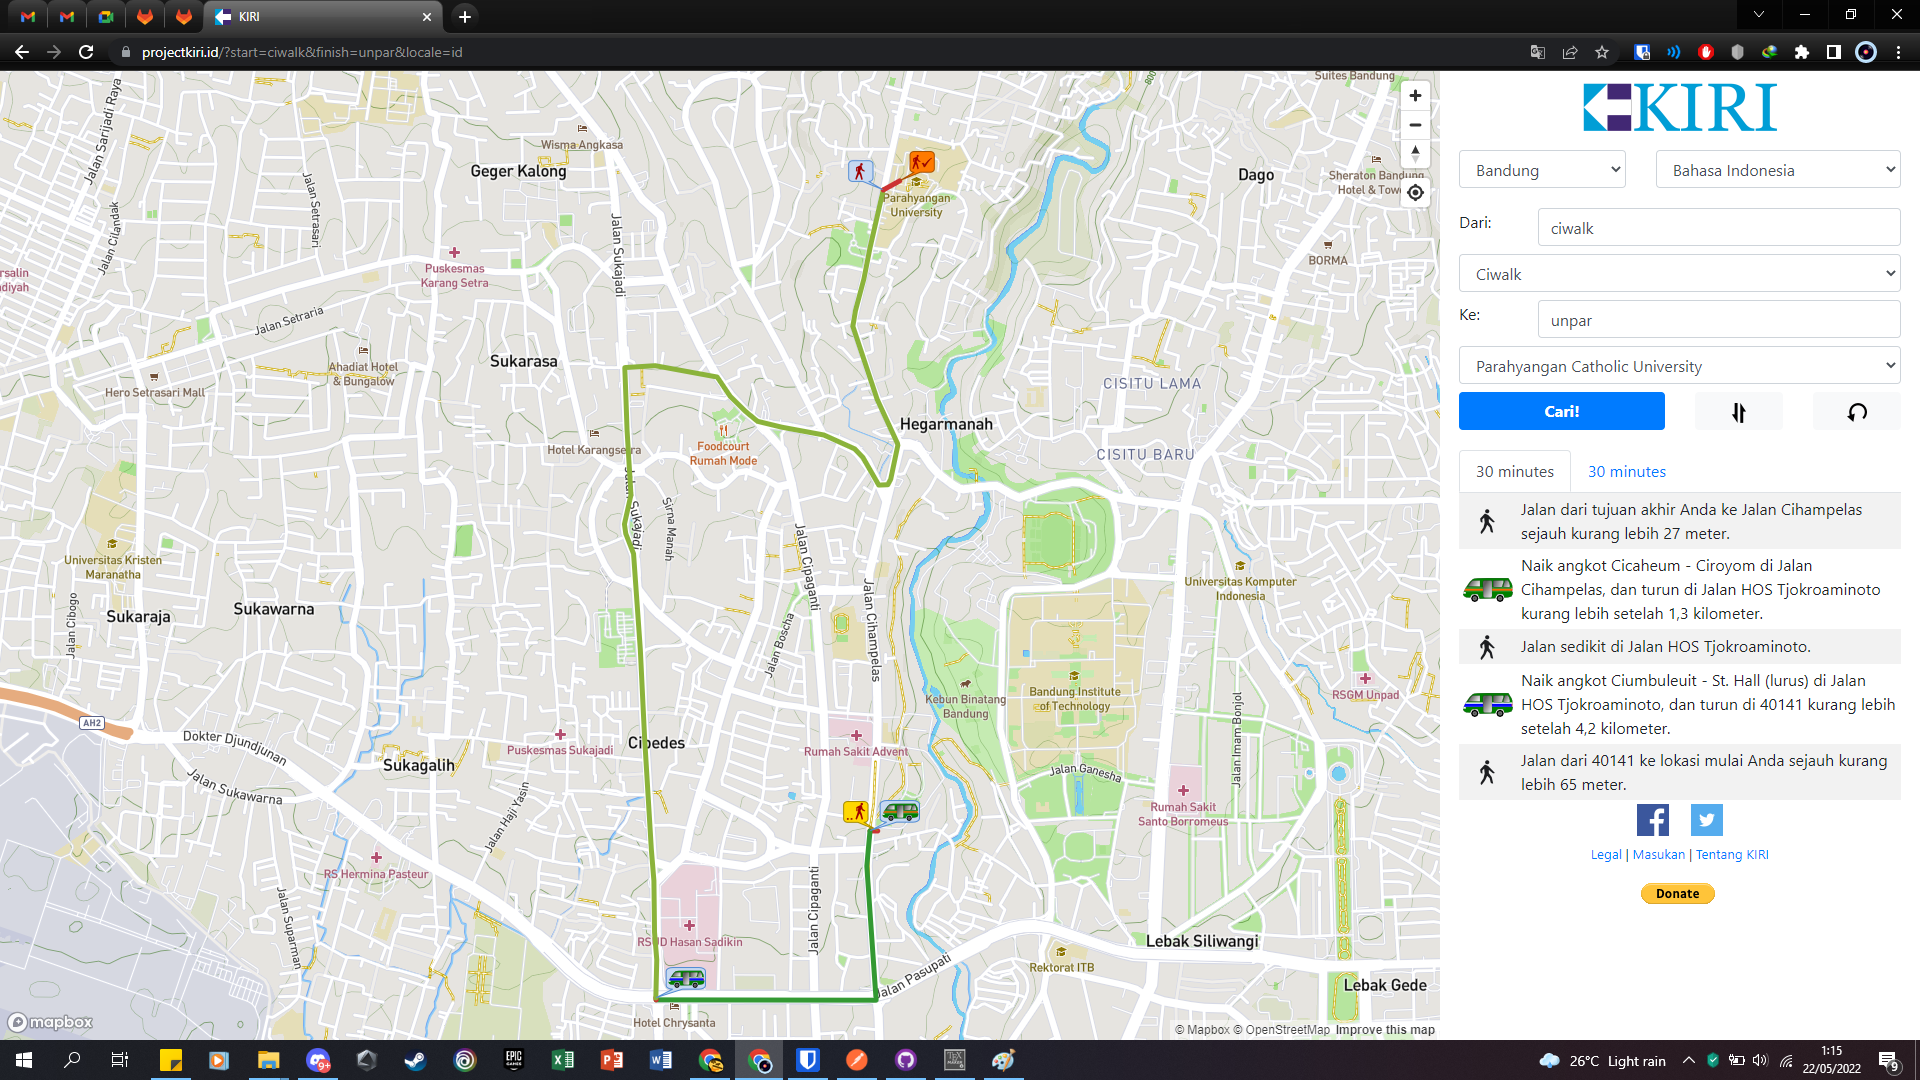
\includegraphics[width=0.74\linewidth]{apikiri-smartdirections}
    \caption[Penggunaan API KIRI untuk layanan \textit{smart direction}]{Penggunaan API KIRI untuk layanan \textit{smart direction}, dari Cihampelas Walk ke UNPAR.}
    \label{fig:kiri-api-smartdirections-usage}
\end{figure}

\section{Fungsi dan \textit{Library} Bahasa C}
\label{sec:cmodules}

Di bagian ini akan dilakukan studi literatur terhadap seluruh fungsi bawaan serta \textit{library-library} bahasa pemrograman C yang akan digunakan dalam pebuatan perkakas ini.

\subsection{getopt \cite{loosemore:2022:gnuclibrary}}
\label{sec:cmodules-getopt}

\verb|getopt| merupakan sebuah fungsi yang dapat mengautomasi pekerjaan-pekerjaan yang berhubungan dengan penerimaan opsi-opsi untuk \cl berbasis UNIX.
\newline\newline\noindent
Fungsi \verb|getopt| dapat dipanggil dengan format sebagai berikut.

\begin{verbatim}
                         getopt (argc, argv, <options>)
\end{verbatim}

Seluruh kode ini dapat dimasukkan ke suatu variabel berupa sebuah karakter yang merepresentasikan opsi yang ingin digunakan. \verb|argc| merupakan jumlah argumen yang terdapat dalam masukan, sedangkan \verb|argv| merupakan sebuah \textit{array} yang berisi argumen-argumen tersebut.
\newline\newline
Selain itu, penggunaan \verb|getopt| juga akan memakai variabel-variabel tertentu, yang nilainya akan diisi oleh fungsi \verb|getopt| tersebut sendiri. Variabel-variabel ini beserta penjelasannya dapat dilihat di daftar berikut.\footnote{\href{https://www.gnu.org/software/libc/manual/html\_node/Using-Getopt.html}{https://www.gnu.org/software/libc/manual/html\_node/Using-Getopt.html}}
\begin{itemize}
	\item \verb|opterr|\\
	Isi dari variabel ini akan memberi sinyal ke perangkat lunak/perkakas yang menentukan apakah \verb|getopt| akan mengirim pesan ke \textit{error stream} atau tidak. Jika variabel ini bukan bernilai 0, maka pesan \textit{error} akan dikirim. Sebaliknya, jika variabel ini bernilai 0, \verb|getopt| tidak akan mengirim pesan \textit{error} apapun, tetapi tetap akan mengembalikan sebuah karakter tanda tanya (\verb|?|) sebagai tanda bahwa sebuah \textit{error} telah terjadi.
	\item \verb|optopt|\\
	Ketika \verb|getopt| menemukan sebuah karakter yang tidak didefinisikan dalam kumpulan opsi, atau sebuah opsi yang tidak disertai argumen yang diperlukan, karakter tersebut akan disimpan di variabel ini.
	\item \verb|optind|\\
	Variabel ini digunakan oleh \verb|getopt| sebagai indeks untuk \textit{array} \verb|argv|. Jika seluruh argumen sudah diproses, nilai variabel ini dapat digunakan untuk menentukan argumen mana yang merupakan arguman tambahan yang tidak terpakai. Nilai dari variabel ini dimulai dari 1.
	\item \verb|optarg|\\
	Jika opsi yang sedang diproses memerlukan argumen, variabel ini adalah tempat dimana argumen tersebut akan disimpan.
	\item \verb|<options>|\\
	Variabel ini merupakan salah satu variabel yang tertera di format pemanggilan \verb|getopt| diatas. Variabel ini berupa \textit{string} yang menandakan karakter-karakter apa saja yang menjadi opsi yang mungkin dalam perkakas tersebut, beserta tipenya. Jika karakter opsi:
	
	\begin{itemize}
		\item Diikuti dengan titik dua (\verb|:|), maka opsi tersebut memiliki argumen yang bersifat wajib.
		\item Diikuti dengan titik dua ganda (\verb|::|), maka opsi tersebut memiliki argumen yang bersifat opsional.
		\item Tidak diikuti apa-apa, maka opsi tersebut merupakan opsi tidak berarguman.
	\end{itemize}
	
\end{itemize}
\noindent
Untuk memberikan gambaran yang lebih baik mengenai penggunaan fungsi \verb|getopt|, berikut merupakan contoh perangkat lunak berbasis \cl sederhana yang menggunakan fungsi tersebut. Perangkat lunak ini akan menerima masukan berupa opsi tidak berparameter \verb|-a| dan/atau opsi berparameter \verb|-b|. Untuk opsi \verb|-a|, perangkat lunak ini akan mengeluarkan nilai 0 jika opsi \verb|-a| tidak dipakai, dan 1 jika opsi tersebut dipakai. Sebagai keluaran keduanya, perangkat lunak ini akan mengeluarkan isi parameter dari opsi \verb|-b|, atau \verb|NULL| jika opsi \verb|-b| tidak dipakai.

\begin{lstlisting}[language=C, caption=Contoh sederhana penggunaan getopt, label=code:getopt-usage]
#include <ctype.h>
#include <stdio.h>
#include <stdlib.h>
#include <unistd.h>

int main(int argc, char **argv) {
    int aflag = 0;
    char *bvalue = NULL;
    int index;
    int args;

    opterr = 0;

    while ((args = getopt(argc, argv, ":ab:")) != -1)
        switch (args) {
	        case 'a':
	            aflag = 1;
	            break;
	        case 'b':
	            bvalue = optarg;
	            break;
	        case ':':
    	        if (optopt == 'b') {
	                fprintf(stderr, "Option -%c requires an argument.\n", optopt);
	            }
	            return 1;
	        case '?':
	            if (isprint(optopt)) {
	                fprintf(stderr, "Unknown option `-%c'.\n", optopt);
	            }
	            else fprintf(stderr, "Unknown option character `\\x%x'.\n", optopt);
	            return 1;
	        default:
	            abort();
        }

    printf("aflag = %d, bvalue = %s\n", aflag, bvalue);
    for (index = optind; index < argc; index++)
        printf("Non-option argument %s\n", argv[index]);

    return 0;
}
\end{lstlisting}

\subsubsection{getopt-long}
\label{sec:cmodules-getopt-long}

Ada pula versi \verb|getopt| yang memungkinkan perangkat lunak untuk menerima dua jenis opsi\textemdash opsi versi pendek berupa sebuah karakter singular, seperti pada \verb|getopt| biasa, dan/atau opsi panjang bergaya GNU, berupa sebuah kata. Perlu diingat juga bahwa perkakas yang menerima opsi sebagai masukannya sebaiknya memiliki versi panjang dari opsi-opsi tersebut, karena tidak hanya hal ini tidak sulit untuk diimplementasikan, tetapi implementasi versi panjang dari opsi-opsi yang ada juga akan memudahkan pengguna untuk mengingat cara kerja perkakas tersebut.

\verb|getopt-long| juga memiliki seluruh variabel-variabel yang dimiliki oleh \verb|getopt|, hanya saja \verb|getopt-long| memiliki sebuah variabel tambahan berupa struktur, yaitu \verb|long_options|. Variabel ini merupakan sebuah struktur berupa \textit{array} yang berisi beberapa \textit{array} lainnya, di mana \textit{array-array} lain in merupakan masing-masing opsi dari fungsi \verb|getopt-long| tersebut. Tiap-tiap \textit{array} tersebut memiliki variabel-variabel berikut:

\begin{itemize}
	\item \verb|name|\\
	Variabel ini merupakan nama panjang dari opsi.
	\item \verb|has_arg|\\
	Variabel ini merupakan penanda apakah opsi memerlukan argumen atau tidak. Nilai untuk variabel ini adalah \verb|no_argument|, \verb|required_argument|, atau \verb|optional_argument|.
	\item \verb|flag| \& \verb|val|\\ 
	Kedua variabel ini menandakan bagaimana sebuah opsi akan diberlakukan ketika diterima oleh \verb|getopt-long|. Variabel \verb|flag| dapat diisi dengan penunjuk (\textit{pointer}) ke suatu variabel lain yang akan diisi dengan isi dari variabel \verb|val| untuk menandakan bahwa \verb|getopt-long| telah berhasil memroses opsi tersebut. Di lain sisi, jika variabel ini berisi \textit{null pointer}, maka fungsi \verb|getopt-long| akan mengembalikan isi dari variabel \verb|val|.
\end{itemize}
\noindent
Struktur ini harus diakhiri dengan sebuah \textit{array} tambahan yang seluruh variabelnya bernilai 0.
\newline\newline
Untuk menjelaskan lebih lanjut mengenai cara penggunaan \verb|getopt-long|, berikut merupakan contoh perangkat lunak berbasis \cl sederhana yang menggunakan fungsi tersebut. Adapun perangkat lunak ini memiliki spesifikasi sebagai berikut:

\begin{itemize}
	\item Perangkat lunak ini akan menerima masukan dari penggunaan opsi-opsi serta parameternya.
	\item Keluaran dari perangkat lunak ini adalah opsi apa saja yang dipilih, serta parameter yang diberikan (jika ada).
	\item Opsi pertama yang disediakan adalah \verb|-a| atau \verb|--args| yang merupakan opsi tidak berargumen.
	\item Opsi kedua yang disediakan adalah \verb|-n| atau \verb|--noargs|, yang merupakan opsi yang membutuhkan sebuah argumen.
	\item Opsi ketiga dan keempat merupakan penanda mode keluaran, yaitu \verb|--short| dan \verb|--long|. Jika opsi \verb|--long| digunakan, maka perangkat lunak ini akan mengeluarkan versi panjang dari keluaran, sedangkan jika opsi \verb|--short| digunakan, maka perangkat akan mengeluarkan versi pendek dari keluaran.
\end{itemize}

\begin{lstlisting}[language=C, caption=Contoh sederhana penggunaan getopt-long, label=code:getopt-usage-long]
#include <stdio.h>
#include <stdlib.h>
#include <getopt.h>

int main(int argc, char **argv) {
    int option;
    static int verbose;

    while (1) {
        static struct option long_options[] = {
                {"long", 0, &verbose, 1},
                {"short", 0, &verbose, 0},
                {"noargs", 0, 0, 'n'},
                {"args", 1, 0, 'a'},
                {0, 0, 0, 0}};
        int option_index = 0;
        option = getopt_long(argc, argv, "na:", long_options, &option_index);

        if (option == -1)
            break;
        switch (option) {
	        case 0:
    	        if (verbose) {
	                printf("Print mode is set to: %s", long_options[option_index].name);
	            }
	            else
	                printf("Print mode is set to: %s", long_options[option_index].name);
	            putchar('\n');
	            break;

    	    case 'n':
	            if (verbose == 1) {
	                printf("Option '%s' was picked. This option does not require any arguments.", long_options[option_index].name);
    	        }
	            else
	                printf("Argumentless option '%s' was picked.", long_options[option_index].name);
	            putchar('\n');
	            break;

    	    case 'a':
	            if (verbose == 1) {
	                printf("Option '%s' was picked with argument '%s'.", long_options[option_index].name, optarg);
	            }
	            else
	                printf("a = %s", optarg);
	            putchar('\n');
	            break;

    	    case '?':
	            break;
	
	        default:
	            abort();
        }
    }

    if (optind < argc)
    {
        printf("Arguments passed without a corresponding option (argv): ");
        while (optind < argc) {
            printf("%s ", argv[optind++]);
        }
        putchar('\n');
    }

    exit(0);
}
\end{lstlisting}

\subsection{libcurl \cite{stenberg:2022:everythingcurl}}
\label{sec:cmodules-libcurl}

libcurl merupakan sebuah \textit{library} yang berisi fungsi-fungsi yang disediakan dalam bentuk API bahasa C, untuk digunakan oleh aplikasi-aplikasi bahasa C. Libcurl didesain dengan berorientasi transfer (biasanya transfer berkas), tanpa memerlukan para penggunanya untuk mengerti protokol-protokol yang digunakan dalam proses pentransferan tersebut. Fitur transfer ini dapat dibuat sesederhana mungkin, dan seluruh aturan dan opsi seputar pemindahan berkas tersebut dapat diatur nantinya secara manual melalui opsi-opsi yang ada.

Untuk mulai melakukan transfer berkas, diperlukan juga sebuah \textit{handle} yang perlu diinisialisasi terlebih dahulu. Adapun cURL memiliki dua jenis \textit{handle}, yaitu \textit{easy handle} dan \textit{multi handle}. 

\subsubsection{\textit{Easy Handle}}
\label{sec:cmodules-libcurl-handleeasy}

\textit{Easy handle} dari cURL dapat diinisialisasi dengan memanggil fungsi \verb|curl_easy_init()|. Setelah itu, untuk mengatur opsi-opsi yang perlu diatur sesuai kebutuhan pengguna, seperti URL yang dituju, protokol yang ingin dipakai, koneksi ke port spesifik, dan sebagainya,\footnote{\href{https://curl.se/libcurl/c/curl\_easy\_setopt.html}{https://curl.se/libcurl/c/curl\_easy\_setopt.html}} pengguna harus mengaturnya dengan fungsi \verb|curl_easy_setopt()|. \textit{Handle} ini berhasil diatur opsinya apabila fungsi \verb|curl_easy_setopt()| tadi mengembalikan \verb|CURLE_OK|. Terakhir, untuk menjalankan transfernya, fungsi yang perlu dipanggil adalah \verb|curl_easy_perform(<easy handle>)|, dengan variabel \verb|<easy handle>| diisi dengan nama dari \textit{easy handle} yang ingin dimulai transfernya.

\textit{Handle} yang telah diatur ini dapat digunakan berulang kali dengan konfigurasi yang sama, sampai entah pengguna mengganti konfigurasi opsi-opsinya kembali, atau atau \textit{handle}-nya direset dengan pemanggilan fungsi \verb|curl_easy_reset()|.

\subsubsection{\textit{Multi Handle}}
\label{sec:cmodules-libcurl-handlemulti}

\textit{Multi handle} merupakan sebuah \textit{handle} yang dapat memfasilitasi beberapa transfer yang dilakukan secara paralel. Metode pentransferan filenya masih sama dengan \textit{easy handle}, hanya saja untuk \textit{multi handle}, diperlukan sebuah \textit{handle} tambahan yang dapat menampung seluruh \textit{easy handle} yang akan digunakan. Adapun \textit{handle} tipe ini dapat diinisialisasi dengan memanggil fungsi \verb|curl_multi_init()|, dan untuk mengatur opsi-opsi seputar \textit{multi handle} tersebut, pengguna dapat memanggil fungsi \verb|curl_multi_setopt()|.

Untuk memulai transfer paralel, tentunya perlu diinisialisasi dulu masing-masing \textit{easy handle}-nya. Setelah \textit{handle-handle} tersebut diinisialisasi, \textit{handle} tersebut dapat dimasukkan ke dalam sebuah \textit{multi handle} dengan memanggil fungsi berikut.

\begin{verbatim}
              curl_multi_add_handle(<multi handle>, <easy handle>);
\end{verbatim}
\noindent
Dengan \verb|<easy handle>| merupakan nama dari \textit{easy handle} yang ingin dimasukkan ke dalam \textit{multi handle} tertentu dan \verb|<multi handle>| merupakan nama dari \textit{multi handle}-nya sendiri. Sedangkan, untuk menghapus sebuah \textit{easy handle} dari dari dalam \textit{multi handle}, dapat dipanggil fungsi berikut.

\begin{verbatim}
             curl_multi_remove_handle(<multi handle>, <easy handle>);
\end{verbatim}

Setelah seluruh \textit{easy handle} yang ingin dijalankan dimasukkan ke dalam \textit{multi handle}, \textit{multi handle} tersebut dapat dijalankan dengan menggunakan sebuah \textit{loop} transfer. Adapun isi dari loop ini meliputi tiga langkah utama, yaitu:

\begin{enumerate}
	\item Inisialisasi variabel \verb|transfers_running|\\
	\verb|transfers_running| merupakan sebuah variabel \textit{integer} yang menjadi penanda bagi pengguna mengenai berapa banyak \textit{handle} yang sedang melakukan proses transfer di suatu waktu. Selama nilai variabel ini bukan 0, artinya ada \textit{easy handle} yang belum selesai melakukan proses transfer berkas.
	\item Menjalankan transfer dalam \textit{multi handle}\\
	Langkah selanjutnya adalah menjalankan transfer dalam \textit{mutli handle}, dengan memanggil fungsi \verb|curl_multi_perform|. Adapun fungsi tersebut harus dipanggil dengan format berikut, yaitu:

\begin{verbatim}
           curl_multi_perform(<multi handle>, <transfers_running>)
\end{verbatim}

	\item Menunggu transfer untuk selesai sebelum data diekstraksi\\
	Tentunya sebelum data hasil transfer dapat diekstraksi untuk dipakai, proses transfernya sendiri harus selesai terlebih dahulu\textemdash untuk kasus dalam \textit{multi handle} libcurl, seluruh \textit{handle} di dalam \textit{multi handle} harus selesai melakukan transfer terlebih dahulu, atau sampai terjadi \textit{timeout}. Adapun langkah ini dapat diselesaikan entah dengan menggunakan \verb|curl_multi_wait()| atau \verb|curl_multi_poll()|, atau dengan cara manual, yaitu dengan memasukkan deskriptor-deskriptor file serta nilai \textit{timeout} secara manual, dan kemudian menggunakan \verb|select()|, walaupun metode ini tidak dianjurkan karena keterbatasan jumlah deskriptor yang dapat digunakan.\footnote{\href{https://curl.se/libcurl/c/curl\_multi\_poll.html}{https://curl.se/libcurl/c/curl\_multi\_poll.html}}
\end{enumerate}
\noindent
Implementasi singkat dari ketiga langkah ini dapat dilihat di potongan kode berikut.

\begin{lstlisting}[language=C, caption=Loop sederhana dari pengunaan \textit{multi handle} curl, label=code:curl-usage-multi]
do {
   curl_multi_wait (multi_handle, NULL, 0, 1000, NULL);
   curl_multi_perform (multi_handle, &transfers_running);
} while (transfers_running);
\end{lstlisting}

\subsubsection{\textit{Multi Socket Handle}}
\label{sec:cmodules-libcurl-handlemultisocket}

Ada mode lain dari \textit{multi handle}, yaitu \textit{multi socket handle}. Bedanya dengan \textit{multi handle} biasa adalah \textit{multi socket handle} memperhatikan \textit{socket-socket} yang ada dan memberitahu \textit{handle-handle} jika ada \textit{socket} yang sudah siap untuk digunakan dalam proses \textit{read/write}. Cara operasinya hampir sama dengan \textit{multi handle}\textemdash hal utama yang berbeda adalah dengan \textit{multi socket handle}, diperlukan satu buah parameter tambahan, yaitu kumpulan \textit{socket} yang ingin diperhatikan.

\textit{Socket} ini, beserta apa aksi yang ingin ditunggu dalam socket tersebut, diperhatikan dengan implementasi sebuah fungsi \textit{callback}, yaitu \verb|socket_callback()|. Handle mana yang ingin digunakan, socket mana yang ingin diperhatikan, serta aksi apa yang ditunggu diatur dalam fungsi ini. Jika ada beberapa \textit{socket} yang ingin diperhatikan, fungsi ini harus dipanggil lagi untuk setiap \textit{socket}-nya. Selain itu, perlu juga dipanggil fungsi \verb|timer_callback()|, yang berfungsi untuk mengatur seberapa lama aplikasi akan menunggu \textit{socket}, sebelum terjadi \textit{timeout}. Kedua \textit{callback} ini dapat diatur ke dalam suatu \textit{multi handle} dengan menggunakan fungsi \verb|curl_multi_setopt()| biasa\textemdash untuk \textit{callback socket}, fungsi ini ditandai dengan menggunakan paramter \verb|CURLMOPT_TIMERFUNCTION|, sedangkan untuk \textit{callback timer}, fungsi tersebut ditandai dengan parameter \verb|CURLMOPT_TIMERFUNCTION|.

Adapun seluruh \textit{handle} ini dapat dipanggil dengan memanggil fungsi \verb|curl_multi_socket_action()|, dan cara untuk melihat apakah seluruh transfer sudah selesai atau masih ada transfer yang berlangsung pada suatu waktu sama dengan \textit{multi transfer} biasa.

Contoh implementasi singkat dari seluruh fungsi-fungsi tersebut dapat dilihat di potongan kode berikut.

\begin{lstlisting}[language=C, caption=Kumpulan implementasi pengunaan \textit{multi socket handle} curl, label=code:curl-usage-multisocket]
/* socket callback */
int socket_callback(CURL *easy,      /* easy handle */
                    curl_socket_t s, /* socket */
                    int what,        /* aksi apa yang ditunggu */
                    void *userp,     /* penunjuk callback privat */
                    void *socketp)   /* penunjuk socket privat */

curl_multi_setopt(multi_handle, CURLMOPT_SOCKETFUNCTION, socket_callback);

/* timer callback */
int timer_callback(multi_handle,   /* multi handle */
                   timeout_ms,     /* waktu tunggu dalam milidetik */
                   userp)          /* penunjuk callback privat */

curl_multi_setopt(multi_handle, CURLMOPT_TIMERFUNCTION, timer_callback);

/* multi socket action */
curl_multi_socket_action(multi, CURL_SOCKET_TIMEOUT, 0, &running);
\end{lstlisting}

\subsection{cJSON\protect\footnotemark}
\label{sec:cmodules-cJSON}
\footnotetext{\href{https://github.com/DaveGamble/cJSON}{https://github.com/DaveGamble/cJSON}}

cJSON merupakan sebuah \textit{library} yang berfungsi sebagai \textit{parser} JSON untuk perangkat-perangkat lunak bahasa C. \textit{Library} ini sendiri terdiri atas sebuah file C dan sebuah file header.

\subsubsection{Instalasi}
\label{sec:cmodules-cJSON-instalation}

cJSON dapat diinstal dengan beberapa cara, yaitu:

\begin{itemize}[listparindent=\parindent]
	\item Manual\\
	Instalasi manual hanya membutuhkan pengembang perangkat lunak untuk menyalin kedua file \textit{library} cJSON ke dalam direktori perangkat lunak tersebut.
	\item CMake\\
	Untuk penggunaan cJSON dengan CMake, perlu dibuat sebuah direktori bernama \verb|build|, dan kemudian CMake harus dijalankan di dalam direktori tersebut, dengan mengeksekusi perintah \verb|cmake|. Dengan melakukan ini, Makefile akan dibuat di dalam direktori tersebut, yang nantinya akan dapat di-\textit{compile} dan diinstal dengan perintah \verb|make install|, atau \verb|cmake --install|. Selain file-file \textit{header} dan \textit{library}, proses ini juga akan menginstal file-file untuk \verb|pkg-config|, untuk memudahkan deteksi instalasi CMake sebelumnya.
	
	Proses pembangunan cJSON juga memiliki beberapa opsi yang dapat diatur sedemikian rupa sesuai dengan kebutuhan pembuat perangkat lunak. Adapun opsi-opsi yang dapat diatur dapat dilihat di daftar berikut.

	\begin{itemize}
		\item \verb|-DENABLE_CJSON_TEST|\\
		\textbf{Nilai awal:} On\\
		Jika opsi ini dinyalakan (diberi nilai ``On``), maka tes-tes cJSON akan dibuat dan dijalankan bersamaan dengan instalasi.
		\item \verb|-DENABLE_CJSON_UTILS|\\
		\textbf{Nilai awal:} Off\\
		Jika opsi ini dinyalakan, maka file-file utilitas cJSON akan diinstal bersamaa dengan proses instalasi utama.
		\item \verb|-DENABLE_TARGET_EXPORT|\\
		\textbf{Nilai awal:} On\\
		Mengekspor target-target ekspor cJSON. Opsi ini dapat dimatikan jika terjadi masalah saat instalasi.
		\item \verb|-DENABLE_CUSTOM_COMPILER_FLAGS|\\
		\textbf{Nilai awal:} On\\
		Mengaktifkan properti-properti untuk \textit{compiler} non-standar (Clang, GCC, MSVC). Opsi ini dapat dimatikan jika terjadi masalah saat instalasi.
		\item \verb|-DENABLE_VALGRIND|\\
		\textbf{Nilai awal:} Off\\
		Menjalankan tes-tes yang ada menggunakan \mbox{Valgrind}.
		\item \verb|-DENABLE_SANITIZERS|\\
		\textbf{Nilai awal:} Off\\
		Meng-\textit{compile} cJSON dengan menyalakan \mbox{AddressSanitizer} dan \mbox{UndefinedBehaviorSanitizer}.
		\item \verb|-DENABLE_SAFE_STACK|\\
		\textbf{Nilai awal:} Off\\
		Menyalakan SafeStack. Pada saat skripsi ini dibuat, fitur ini hanya didukung untuk \textit{compiler} Clang.
		\item \verb|-DBUILD_SHARED_LIBS|\\
		\textbf{Nilai awal:} Off\\
		Membangun semua \textit{shared library} yang tersedia.
		\item \verb|-DBUILD_SHARED_AND_STATIC_LIBS|\\
		\textbf{Nilai awal:} On\\
		Membangun \textit{shared library} dan \textit{static library} yang tersedia.
		\item \verb|-DCMAKE_INSTALL_PREFIX|\\
		\textbf{Nilai awal:} -\\
		Mengatur \textit{prefix} direktori tempat instalasi cJSON.
		\item \verb|-DENABLE_LOCALES|\\
		\textbf{Nilai awal:} On\\
		Memungkinkan penggunaan metode \verb|localeconv|.
		\item \verb|-DCJSON_OVERRIDE_BUILD_SHARED_LIBS|\\
		\textbf{Nilai awal:} On\\
		Memungkinkan penimpaan nilai dari opsi \verb|-BUILD_SHARED_LIBS| menggunakan nilai dari opsi \verb|-DCJSON_BUILD_SHARED_LIBS|.
		\item \verb|-DENABLE_CJSON_VERSION_SO|\\
		\textbf{Nilai awal:} On\\
		Menyalakan versi so dari cJSON.
	\end{itemize}

	\item Makefile\\
	Jika CMake tidak tersedia, cJSON juga dapat dibangun dengan menggunakan GNU Make, dengan menggunakan perintah \verb|make all|, dan menginstal \textit{library-library} yang sudah ter-\textit{compile} dengan perintah \verb|make install|. Akan tetapi, perlu diingat bahwa metode instalasi ini sudah tidak lagi diperbarui (\textit{deprecated}), dan dukungannya hanya sebatas pembetulan \textit{bug}.
	
	\item vcpkg\\
	Melalui vcpkg, cJSON dapat diunduh dan diinstal secara langsung. Versi vcpkg dari cJSON terus diperbarui oleh tim Microsoft dan kontributor-kontributor dari komunitas publik, jadi \textit{library} cJSON yang diinstal melalui vcpkg kemungkinan besar akan selalu merupakan versi terbarunya.
\end{itemize}

\subsubsection{Penggunaan}
\label{sec:cmodules-cJSON-usage}

Jika cJSON diinstal melalui CMake atau Makefile, cJSON dapat digunakan dengan mengikutkan baris ini dalam kode program:

\begin{verbatim}
                             #include <cjson/cJSON.h>
\end{verbatim}

\subsubsection{Struktur Data}
\label{sec:cmodules-cJSON-datastruct}

cJSON merepresentasikan sebuah nilai JSON dengan struktur data \verb|cJSON|, yang dapat dilihat di potongan kode \ref{code:cjson-struct}.

\begin{lstlisting}[caption=Struktur data cJSON, label=code:cjson-struct]
typedef struct cJSON
{
    struct cJSON *next;
    struct cJSON *prev;
    struct cJSON *child;
    int type;
    char *valuestring;
    int valueint;
    double valuedouble;
    char *string;
} cJSON;
\end{lstlisting}
\noindent
Dengan variabel-variabel dalam struktur tersebut sebagai berikut:

\begin{itemize}
	\item \verb|next| dan \verb|prev|\\
	Variabel ini merupakan penunjuk ke struktur cJSON lainnya yang merupakan nilai JSON selanjutnya (untuk \verb|next|) dan sebelumnya (untuk \verb|prev|).
	\item \verb|child|\\
	Variabel ini merupakan penunjuk ke struktur cJSON lainnya yang merupakan elemen JSON di dalam struktur cJSON tersebut.
	\item \verb|type|\\
	Variabel ini menandakan tipe dari nilai JSON yang terdapat di dalam struktur cJSON tersebut. Adapun tipe-tipe yang mungkin adalah sebagai berikut.
	
	\begin{itemize}
		\item \verb|cJSON_Invalid|\\
		Merepresentasikan sebuah objek yang tidak valid dan tidak bernilai. Jika seluruh \textit{field} diatur sehingga panjangnya 0 \textit{byte}, maka variabel \verb|type| akan otomatis berisi tipe ini.
		\item \verb|cJSON_True|\\
		Merepresentasikan nilai booolean \textit{true}.
		\item \verb|cJSON_False|\\
		Merepresentasikan nilai booolean \textit{false}.
		\item \verb|cJSON_Number|\\
		Merepresentasikan nilai numerik apapun. Jika nilainya merupakan nilai \textit{double}, maka nilai tersebut akan disimpan di dalam variabel \verb|valuedouble|. Sedangkan jika nilainya merupakan nilai \textit{integer}, maka nilai tersebut akan disimpan di dalam variabel \verb|valueint|.
		\item \verb|cJSON_String|\\
		Merepresentasikan nilai \textit{string} apapun. Nilainya disimpan sebagai \textit{string} yang dipisah dengan \textit{null terminator} ('\verb|\0|' atau \verb|\u0000|).
		\item \verb|cJSON_Array|\\
		Merepresentasikan nilai \textit{array}. \textit{Array} dalam cJSON diimplementasikan dengan menunjukkan isi dari variabel \verb|child| tadi ke sebuah \textit{linked list} dari objek-objek cJSON. Jika objek cJSON ini merupakan elemen dalam sebuah \textit{array}, maka isi dari variabel \verb|prev| dan \verb|next| merupakan salah satu dari elemen-elemen lain dalam \textit{array} yang menjadi elemen sebelum dan sesudah elemen ini.
		\item \verb|cJSON_Object|\\
		Merepresentasikan nilai objek general. Implementasinya sama dengan \textit{array}, hanya saja untuk objek general, kuncinya diletakkan di dalam variabel \verb|string|.
		\item \verb|cJSON_Raw|\\
		Merepresentasikan objek JSON apapun yang disimpan dalam bentuk \textit{array} yang diterminasi/dipisah oleh \textit{null terminator}.
		\item \verb|cJSON_NULL|\\
		Merepresentasikan sebuah nilai \textit{null}.
	\end{itemize}
	
	\item \verb|valuestring|/\verb|valuestring|/\verb|valuestring|/\verb|string|\\	
	Merupakan variabel-variabel yang menyimpan nilai dari struktur cJSON. Variabel apa yang diisi dan apa isinya tergantung dari tipe data yang disimpan.
\end{itemize}

\subsubsection{Fungsi-Fungsi Dasar}
\label{sec:cmodules-cJSON-basicfuncts}

\begin{itemize}[listparindent=\parindent]
	\item Tipe-tipe data dasar\\
	Untuk setiap tipe data cJSON, ada sebuah fungsi \verb|cJSON_Create...|. Semua fungsi \mbox{tersebut} akan mengalokasikan sebuah struktur cJSON yang nantinya dapat dihapus dengan \verb|cJSON_Delete|. Perlu diingat juga bahwa seluruh struktur yang dibuat harus dihapus agar tidak terjadi kebocoran memori. Adapun fungsi-fungsi \verb|cJSON_Create| yang dapat digunakan untuk tipe-tipe data yang tersedia adalah sebagai berikut.
	
	\begin{itemize}
		\item \textit{null} dibuat dengan \verb|cJSON_CreateNull|.
		\item \textit{boolean} dibuat dengan \verb|cJSON_CreateBool|, atau jika ingin membuat data \textit{boolean} langsung dengan nilainya, dapat menggunakan \verb|cJSON_CreateTrue| atau \verb|cJSON_CreateFalse|.
		\item Bilangan apapun dibuat dengan \verb|cJSON_CreateNumber|. Penggunaan fungsi ini akan langsung mengisi nilai variabel \verb|valueint| dan \verb|valuedouble|.
		\item \textit{string} apapun dibuat dengan \verb|cJSON_CreateString| (membuat sebuah string langsung sebagai nilai data JSON), atau \verb|cJSON_CreateStringReference| (mereferensikan \textit{string} yang sudah ada sebagai nilai data JSON).
	\end{itemize}
	
	\item \textit{Array}\\
	Sebuah \textit{array} kosong dapat dibuat dengan menggunakan fungsi \verb|cJSON_CreateArray|. Selain fungsi tersebut, pembuatan \textit{array} juga dapat dilakukan dengan memanggil sebuah fungsi alternatif, yaitu \verb|cJSON_CreateArrayReference|. Bedanya adalah dengan fungsi alternatif ini, \textit{array} yang dibuat tidak secara langsung ``mengandung'' nilai-nilainya, jadi ketika \textit{array} tersebut dihapus dengan \verb|cJSON_Delete|, nilai-nilai di dalamnya tidak terhapus juga. Hal yang sama juga dapat dilakukan dengan objek-objek di dalam \textit{array} tersebut, dimana objek ini dapat ditambahkan dengan fungsi \verb|cJSON_AddItemToArray|, yang akan langsung menambahkan objek tersebut ke dalam \textit{array}-nya, atau dengan menggunakan \verb|cJSON_AddItemReferenceToArray|, yang hanya akan menambahkan referensi dari objek yang ingin ditambahkan ke dalam \textit{array}.
	
	Jika ada sebuah objek yang ingin dihapus dari \textit{array} tertentu, perangkat lunak dapat memanggil fungsi \verb|cJSON_DetachItemFromArray|. Fungsi ini akan mengembalikan objek yang dihapus dari \textit{array} tadi, jadi objek ini harus diberikan ke sebuah penunjuk lainnya (dimasukkan ke dalam variabel lain) agar tidak terjadi kebocoran memori. Selain fungsi tersebut, fungsi \verb|cJSON_DeleteItemFromArray| juga dapat digunakan\textemdash bedanya adalah objek yang dihapus dari \textit{array} tadi, jika dihapus menggunakan fungsi ini, akan langsung dihapus, seakan-akan fungsi \verb|cJSON_Delete| dipanggil untuk objek tersebut.
	
	Untuk menimpa/mengganti nilai suatu objek di dalam \textit{array}, fungsi \verb|cJSON_ReplaceItemIn|\linebreak \verb|Array| dapat dipanggil dengan indeks dari objek yang ingin diganti sebagai parameternya. Selain fungsi tersebut, fungsi \verb|cJSON_ReplaceItemViaPointer| juga dapat digunakan\textemdash fungsi ini bekerja dengan memutuskan (\textit{detach}) objek lama yang ingin diganti, menghapus objek tersebut, dan menyisipkan objek yang baru ke tempat objek lama yang sudah dihapus tadi.
	
	Terakhir, untuk mendapatkan objek tertentu dalam \textit{array} berdasarkan indeksnya, \mbox{perangkat} lunak dapat memanggil fungsi \verb|cJSON_GetArrayItem|. Ukuran dari \textit{array}-nya sendiri juga dapat dilihat dengan fungsi \verb|cJSON_GetArraySize|.
	
	\item Objek\\	
	Sama seperti \textit{array}, ada dua jenis fungsi pembuatan objek. Yang pertama adalah \verb|cJSON_Create|\linebreak \verb|Object| untuk membuat objek biasa, dan \verb|cJSON_CreateObjectReference| untuk membuat objek yang nilai-nilainya terdiri atas kumpulan referensi ke variabel-variabel lain.
	
	Untuk menambahkan sebuah objek ke dalam suatu objek lainnya, pengguna dapat \mbox{memanggil} fungsi \verb|cJSON_AddItemToObject|. Jika objek ingin ditambahkan ke suatu \mbox{objek} lain yang memiliki sebuah variabel konstan sebagai nama, atau sebuah referensi, prosesnya harus menggunakan fungsi \verb|cJSON_AddItemToObjectCS|.

	Fungsi \verb|cJSON_DetachItemFromObjectCaseSensitive| dapat dipanggil ketika ada \mbox{sebuah} objek ingin dibuang dari objek lain. Sama seperti fungsi \textit{detach} di \textit{array} tadi, fungsi ini akan mengembalikan objek yang dibuang tadi, dan objek tersebut harus \mbox{dimasukkan} ke variabel lain untuk menghindari kebocoran memori. Selain itu, ada juga fungsi \verb|cJSON_DeleteItemFrom|\linebreak \verb|ObjectCaseSensitive|, yang bekerja dengan cara yang sama seperti fungsi penghapusan objek untuk \textit{array}.

	Untuk pengeditan/penggantian nilai objek, lagi-lagi cara kerjanya sama dengan \textit{array}. \mbox{Untuk} penggantian nilai objek berdasarkan kuncinya, fungsi \verb|cJSON_ReplaceItemInObject|\linebreak \verb|CaseSensitive| dapat digunakan, sedangkan untuk penggantian objek langsung dengan penunjuk ke elemen lainnya, fungsi \verb|cJSON_ReplaceItemViaPointer| dapat digunakan.

	Terakhir, untuk mengakses sebuah benda di dalam objek, pengguna dapat memanggil fungsi \verb|cJSON_GetObjectItemCaseSensitive|, dan untuk mengetahui ukuran dari objek tersebut, fungsi yang dapat digunakan sama dengan fungsi yang dapat digunakan untuk \textit{array}, yaitu \verb|cJSON_GetArraySize|.

	\item \textit{Parsing}\\
	Objek JSON yang dibatasi/diterminasi dengan \textit{null terminator} dapat di-\textit{parse} dengan \mbox{menggunakan} fungsi berikut.
	
	\begin{verbatim}
                            cJSON_Parse(<JSON>)
	\end{verbatim}
	\noindent
	Sedangkan, jika objek JSON tersebut tidak (atau belum tentu) dibatasi oleh \textit{null terminator}, objek tersebut dapat di-\textit{parse} dengan fungsi berikut.
	
	\begin{verbatim}
           cJSON_Parse(<JSON>, <ukuran JSON yang ingin di-parse>)
	\end{verbatim}
	\noindent
	Kedua fungsi ini akan membuat sebuah struktur hierarkial dari objek-objek cJSON yang merepresentasikan keseluruhan dari objek JSON tersebut. Setelah objek ini selesai digunakan, penggunanya harus mendealokasikan objek tersebut dengan fungsi \verb|cJSON_Delete|.
\end{itemize}

\subsection{CMake \cite{kitware:2022:masteringcmake}}
\label{sec:cmodules-CMake}

CMake merupakan sebuah perkakas generator \textit{build system} yang memungkinkan pengembang perangkat lunak untuk menentukan parameter-parameter pembangunan perangkat di sebuah file yang berupa teks biasa. File ini kemudian dipakai oleh CMake untuk membuat perkakas-perkakas pembangunan perangkat lunak yang dapat dibaca oleh IDE-IDE tertentu, seperti Microsoft Visual Studio, Apple Xcode, Linux, dan sebagainya. Selain itu, CMake juga menangani aspek-aspek rumit dari pembangunan perangkat lunak, seperti pembangunan perangkat lunak \textit{cross-platform}, introspeksi sistem, dan juga pembangunan perangkat lunak yang dapat disesuaikan berdasarkan penggunanya.

Untuk proyek-proyek yang dibangun di satu platform, CMake memiliki fungsi sebagai berikut.

\begin{itemize}
	\item Memberikan kemampuan untuk melakukan pencarian seluruh perangkat lunak, file-file \textit{library}, dan file-file \textit{header} yang dibutuhkan untuk proses pembangunan perangkat lunak. Pencarian ini juga dapat dilakukan sampai ke dalam \textit{registry} sistem.
	\item Memungkinkan pembangunan perangkat lunak diluar folder tempat \textit{source code} perangkat lunak tersebut sendiri.
	\item Memberikan kemampuan untuk membuat perintah-perintah khusus untuk file-file yang dibuat secara otomatis, seperti \verb|moc()| dari Qt, atau generator pembungkus dari SWIG. Perintah-perintah ini dapat mengatur pembuatan file \textit{source} baru yang nantinya akan diintegrasikan langsung ke dalam perangkat lunak akhirnya.
	\item Memberikan kemampuan untuk memilihkan file-file opsional dari \textit{library} yang digunakan.
	\item Memungkinkan pengaturan pembuatan proyek dari sebuah file \verb|.txt| sederhana.
	\item Kemampuan untuk dengan mudah beralih dari \textit{static build} dan \textit{shared build}.
	\item Membuat ketentuan keperluan (\textit{dependency}) secara otomatis.
\end{itemize}
\noindent
Sedangkan, untuk perangkat-perangkat lunak yang dibuat \textit{cross-platform}, CMake memberikan fungsi-fungsi tambahan sebagai berikut.

\begin{itemize}
	\item Memberikan kemampuan mengetes urutan \textit{machine byte} dan karakteristik-karakteristik lainnya yang spesifik untuk suatu sistem operasi.
	\item File konfigurasi yang dibuat dapat berlaku untuk seluruh \textit{platform}.
	\item Memberikan dukungan untuk membangun \textit{shared build} untuk seluruh \textit{platform} yang mendukungnya.
	\item Memberikan kemampuan untuk mengatur opsi-opsi yang spesifik untuk suatu sistem operasi, seperti misalnya lokasi file-file data utama.
\end{itemize}

\subsubsection{Penggunaan Dasar}
\label{sec:cmodules-CMake-basicusage}

CMake mengambil satu (atau lebih) file-file CMakeLists sebagai masukan, dan sebagai keluaran akan menghasilkan file-file proyek atau Makefile yang dapat digunakan dengan dan oleh perkakas-perkakas pembangunan perangkat lunak lain yang ada.

Proses CMake umumnya terdiri atas langkah-langkah berikut.

\begin{enumerate}
	\item Proyek yang ingin dibangun didefinisikan di salah satu file CMakeLists.\\
	File-file CMakeLists (yang berupa file-file \verb|.txt|) merupakan file-file \textit{plain text} yang berisi deskripsi proyek dalam bahasa CMake. Tertera di kode \ref{code:cmake-basecode} merupakan file CMakeLists yang dapat digunakan untuk membangun sebuah program \textit{``Hello World''} sederhana dalam bahasa C, sebagai gambaran mengenai hal-hal apa saja yang minimal harus ada di dalam file CMakeLists.
	
	\begin{lstlisting}[caption=Kode utama operasional CMake, label=code:cmake-basecode]
cmake_minimum_required(VERSION 3.20)
project(Hello)
add_executable(Hello Hello.c)
	\end{lstlisting}
	
	Penjelasan dari baris-baris berikut adalah sebagai berikut.
	
	\begin{itemize}
		\item Baris pertama harus selalu merupakan \verb|cmake_minimum_required|. Hal ini mengharuskan proyek untuk menggunakan versi dari CMake yang dispesifikasi, dan juga memungkinkan \textit{backwards compatibility}.
		\item Baris selanjutnya merupakan perintah \verb|project|. Perintah ini mengatur nama proyek, dan juga bisa digunakan untuk mengatur aturan-aturan lainnya, seperti versi, atau bahasa dari proyek.
		\item Terakhir, perintah \verb|add_executable| merupakan sebuah perintah yang akan menambahkan sebuah file \textit{executable} untuk menjalankan proyek yang sudah dibangun tersebut.
	\end{itemize}
	\item CMake membuat dan mengkonfigurasi proyek tersebut.\\
	Setelah file-file CMakeLists selesai dibuat, CMake akan memproses file-file tersebut dan membuat entri-entri dalam sebuah file \textit{cache}. Pengembang perangkat lunak dapat mengedit file CMakeLists atau mengatur isi dari file \textit{cache} tadi dengan GUI CMake, ccmake, atau untuk proyek-proyek skala kecil, langsung dari \cl.
	
	\begin{itemize}
		\item GUI CMake\\
		CMake memiliki perangkat lunak GUI berbasis Qt yang bisa digunakan di sebagian besar sistem operasi, seperti UNIX, Mac OS X, dan Windows. Perangkat lunak ini, \verb|cmake-gui|, sudah terinstal bersama dengan CMake, tetapi membutuhkan instalasi Qt untuk dijalankan. Tampilan dari perangkat lunak ini dapat dilihat di gambar \ref{fig:cmake-gui}.
		
		\begin{figure}[ht]
		    \centering
		    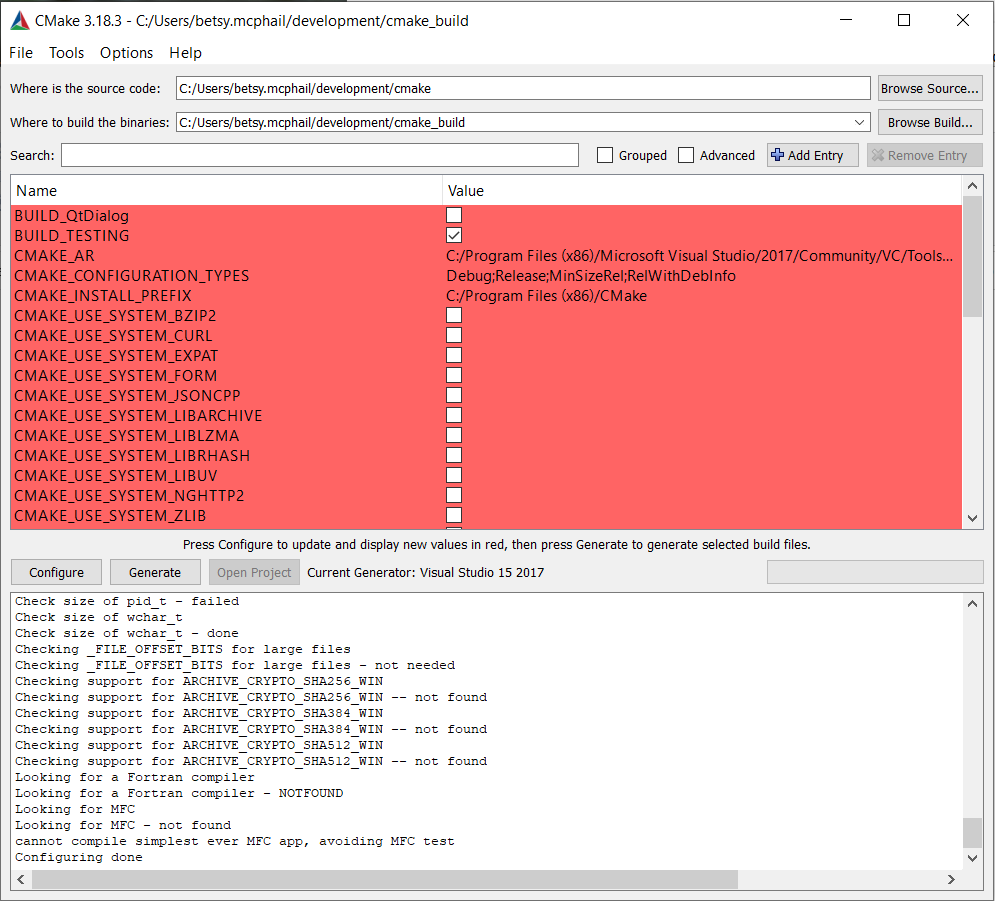
\includegraphics[width=0.66667\linewidth]{cmake-gui}
		    \caption[Tampilan aplikasi cmake-gui]{Tampilan aplikasi cmake-gui.\protect\footnotemark}
		    \label{fig:cmake-gui}
		\end{figure}
		\footnotetext{\href{https://cmake.org/cmake/help/book/mastering-cmake/chapter/Getting\%20Started.html}{https://cmake.org/cmake/help/book/mastering-cmake/chapter/Getting\%20Started.html}}
		
		Dua \textit{field} paling atas adalah direktori dari \textit{source code} dan direktori tempat file-file \textit{binary} nantinya akan diletakkan setelah dibuat. Kedua \textit{field} ini harus diisi secara manual, walaupun jika direktori \textit{binary} ini sudah dikonfigurasi langsung melalui CMake sebelumnya, \textit{field} direktori kedua akan secara otomatis terisi.
%		\newpage % Prevent widow
		\item ccmake\\
		Di mayoritas sistem operasi berbasis UNIX, jika \textit{library curses}	didukung, maka CMake memiliki sebuah perangkat lunak lain yang dapat digunakan, yaitu \verb|ccmake|. Untuk menjalankan \verb|ccmake|, pengguna dapat menjalankannya melalui \textit{command line}, dan direktori tempat \verb|ccmake| dijalankan ini harus merupakan direktori tempat file-file \textit{binary} nantinya ingin disimpan. Ketika aplikasi ini dijalankan, akan keluar tampilan seperti di gambar \ref{fig:cmake-ccmake}. Adapun instruksi singkat penggunaan dari aplikasi ini dapat dilihat di bagian bawah dari tampilan tersebut.
		
		\begin{figure}[ht]
		    \centering
		    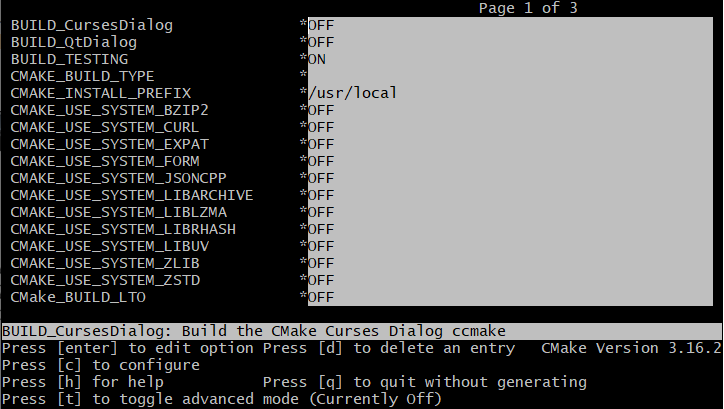
\includegraphics[width=0.66667\linewidth]{cmake-ccmake}
		    \caption[Tampilan aplikasi ccmake]{Tampilan aplikasi ccmake.\protect\footnotemark}
		    \label{fig:cmake-ccmake}
		\end{figure}
		\footnotetext{\href{https://cmake.org/cmake/help/book/mastering-cmake/chapter/Getting\%20Started.html}{https://cmake.org/cmake/help/book/mastering-cmake/chapter/Getting\%20Started.html}}
		
		\item Langsung dari \cl\\
		CMake juga dapat dijalankan melalui \textit{command line}. Untuk menjalankan CMake dari \textit{command line}, direktori tempat terminal berada lagi-lagi harus diatur ke direktori tempat file-file \textit{binary} akan disimpan. Kemudian jalankan perintah \verb|cmake| dengan opsi-opsi yang diinginkan, diikuti dengan direktori tempat \textit{source code} dari perangkat lunak yang ingin dibangun berada. Walaupun begitu, perlu diingat bahwa metode ini direkomendasikan untuk digunakan hanya untuk proyek-proyek yang memiliki sedikit, atau bahkan tidak ada opsi sama sekali.
	\end{itemize}
	
	\item Pengguna membangun proyek tersebut dengan perkakas pembangunan masing-masing.\\
	CMake dapat memberikan beberapa opsi dalam pembangunan perangkat lunak yang dapat diatur oleh penggunanya masing-masing. Adapun dua opsi utama dari seluruh opsi-opsi tersebut adalah sebagai berikut.
	
	\begin{itemize}
		\item Menspesifikasi \textit{compiler} yang akan digunakan\\
		Di beberapa sistem, bisa jadi terdapat lebih dari satu \textit{compiler}, atau \textit{compiler} yang ada tidak berada di tempat \textit{compiler} tersebut biasa diinstal. Di kasus-kasus ini, CMake perlu diberitahu secara manual dimana letak \textit{compiler} yang ingin digunakan. Ada tiga cara untuk melakukan ini, yaitu dengan:
		
		\begin{itemize}
			\item menspesifikasikan \textit{compiler} yang ingin dipakai ke generator,
			\item mengatur variabel \textit{environment}, atau
			\item membuat entri \textit{cache}.
		\end{itemize}
		
		Jika pengaturan \textit{compiler} sudah selesai dan \verb|cmake| sudah dijalankan setidaknya sekali, jika pengguna ingin mengganti \textit{compiler}, pengguna harus memulai ulang dengan folder file \textit{binary} yang kosong.
		\item Mengatur konfigurasi pembangunan perangkat\\
		Konfigurasi pembangunan perangkat memungkinkan sebuah proyek untuk dibangun dalam beberapa cara dengan tujuan \textit{debugging}, optimisasi, atau tujuan-tujuan sejenis lainnya. Secara \textit{default}, CMake mendukung mode-mode berikut:
		
		\begin{itemize}
			\item \verb|Debug|\textemdash Opsi-opsi \textit{debug} dasar dinyalakan.
			\item \verb|Release|\textemdash Fungsi optimisasi dasar dinyalakan.
			\item \verb|MinSizeRel|\textemdash Ukuran kode akhir diusahakan sekecil mungkin.
			\item \verb|RelWithDebinfo|\textemdash Membangun \textit{build} optimal dan mengikutkan informasi-informasi untuk \textit{debugging}.
		\end{itemize}
		
		Dengan generator-generator berbasis Makefile, hanya sebuah mode konfigurasi yang bisa aktif ketika CMake sedang dijalankan, dan mode tersebut diatur dengan variabel \verb|CMAKE_BUILD_TYPE|. Jika variabel ini dikosongkan (atau tidak dimasukkan ke dalam kode), maka mode yang dipakai adalah mode \textit{default}. Di lain kasus, jika pengembang ingin membangun perangkat dalam dua mode yang berbeda, perintah untuk menjalankan CMake (dengan variabel mode konfigurasi masing-masing) harus dijalankan untuk setiap modenya. 
		Misal, jika pengguna ingin membangun perangkat dengan mode \verb|Debug| dan \verb|Release| sekaligus, maka perintah untuk menjalankan CMake harus ditulis seperti dapat dilihat di potongan kode \ref{code:cmake-multibuild}.
%		\newpage % Prevent widow
		\begin{lstlisting}[caption=Contoh kode pembangunan CMake lebih dari satu mode, label=code:cmake-multibuild]
ccmake ../<direktori> -DCMAKE_BUILD_TYPE=Debug
ccmake ../<direktori> -DCMAKE_BUILD_TYPE=Release
		\end{lstlisting}
		
	\end{itemize}
	
	Setelah CMake dijalankan, proyek tersebut siap untuk dibangun. Jika generator yang dipilih merupakan generator berbasis Makefiles, maka proyek tersebut dapat dibangun dengan mengganti \textit{working direktory} ke lokasi file-file \textit{binary}, dan kemudian menjalankan perintah \verb|make| atau \verb|cmake --install|. Jika generator yang dipilih merupakan sebuah IDE, maka proyek tersebut dapat dibangun secara biasa melalui IDE tersebut.
\end{enumerate}